\documentclass[review]{elsarticle}

\usepackage{lineno,hyperref}
\modulolinenumbers[5]

\journal{Computer Physics Communications}

%%%%%%%%%%%%%%%%%%%%%%%
%% Elsevier bibliography styles
%%%%%%%%%%%%%%%%%%%%%%%

\bibliographystyle{elsarticle-num-names}
\sloppy

\usepackage{graphicx}
\usepackage{caption}
\usepackage{subcaption}
\usepackage{amsmath}
\usepackage{amsthm}
\usepackage{color}
\usepackage{ifpdf}
\usepackage{booktabs} % For formal tables
\usepackage{listings}

%\setcopyright{rightsretained}

\newcommand{\up}{\vspace*{-1em}}
\newcommand{\upp}{\vspace*{-0.4em}}
\newcommand{\uppp}{\vspace*{-0.2em}}

\usepackage{hyperref}
\usepackage{float}
\usepackage[utf8]{inputenc}
\usepackage{multirow}
\usepackage{rotating}
\usepackage{setspace}
\usepackage{makecell}
\usepackage{moresize}
\setlength{\textfloatsep}{5pt}
\usepackage{tabularx}
\usepackage{algorithm}
\usepackage{algpseudocode}

\usepackage{booktabs}
%\usepackage{listings}
%\usepackage{paralist}
\usepackage{multirow}
\usepackage{ifpdf}
\usepackage{xspace}
\usepackage{keyval}
\usepackage{color}
\usepackage{nicefrac}
\usepackage{float}

% \theoremstyle{definition}
% \newtheorem{definition}{Definition}[section]

\usepackage{xcolor}
\usepackage{textcomp}

\definecolor{listinggray}{gray}{0.95}
\definecolor{darkgray}{gray}{0.7}
\definecolor{commentgreen}{rgb}{0, 0.4, 0}
\definecolor{darkblue}{rgb}{0, 0, 0.4}
\definecolor{middleblue}{rgb}{0, 0, 0.7}
\definecolor{darkred}{rgb}{0.4, 0, 0}
\definecolor{brown}{rgb}{0.5, 0.5, 0}

% \usepackage[normalem]{ulem}
% \def\cyanuwave{\bgroup \markoverwith{\lower3.5\p@\hbox{\sixly \textcolor{cyan}{\char58}}}\ULon}
% \def\reduwave{\bgroup \markoverwith{\lower3.5\p@\hbox{\sixly \textcolor{red}{\char58}}}\ULon}
% \def\blueuwave{\bgroup \markoverwith{\lower3.5\p@\hbox{\sixly \textcolor{blue}{\char58}}}\ULon}
% \font\sixly=lasy6 % does not re-load if already loaded, so no memory problem.
% \makeatother

% DOI
%\acmDOI{ }

% ISBN
%\acmISBN{ }


% -*- mode: latex; mode: visual-line; fill-column: 9999; coding: utf-8 -*-

\newif\ifdraft
\drafttrue

\usepackage{breakurl}
\usepackage{url}
\usepackage{adjustbox}
\usepackage{amsmath}
\renewcommand{\ttdefault}{pcr}
\usepackage{tabularx}
\usepackage{textcomp}
%\usepackage{natbib}
\setcitestyle{square, comma, numbers,sort&compress, super}
\usepackage{hypernat}
%\bibpunct{}{}{,}{s}{,}{,}
%% Remove brackets from numbering in List of References
\makeatletter
\renewcommand{\@biblabel}[1]{\quad#1.}
\makeatother
%% no space
\setlength{\bibsep}{0pt}

%% use \carriagereturn from dingbats 
% fix LaTeX Error: Command \checkmark already defined.
\let\checkmark\undefined
\usepackage{dingbat}
\usepackage{color}
\definecolor{mauve}{rgb}{0.58,0,0.82}
\definecolor{gray}{rgb}{0.5,0.5,0.5}
\renewcommand{\ttdefault}{pcr}
\usepackage{listings}

% Python style for highlighting
\newcommand\pythonstyle{\lstset{
    language=Python,
    basicstyle=\scriptsize\ttfamily,
    otherkeywords={self},             % Add keywords here
    keywordstyle=\bfseries\color{blue},
    emph={MyClass,__init__},          % Custom highlighting
    emphstyle=\ttfamily\bfseries\color{deepred},    % Custom highlighting style
    stringstyle=\color{mauve},
    commentstyle=\color{gray}\textit,      
    frame=tb,                         % Any extra options here
    showstringspaces=false,           %
    breaklines=true,
    prebreak=\carriagereturn,
    numberstyle=\tiny\color{gray},
    numbers=left,
    stepnumber=1
}}

% Python environment
\lstnewenvironment{python}[1][]
{
\pythonstyle
\lstset{#1}
}
{}

% Python for inline
\newcommand{\pythoninline[1]}{{\pythonstyle\lstinline!#1!}}

\usepackage{xspace}
\newcommand{\NaH}{Na$^{+}$/H$^{+}$\xspace}
\newcommand{\Na}{Na$^{+}$\xspace}
\newcommand{\Hp}{H$^{+}$\xspace}
\newcommand{\pKa}{\ensuremath{\mathrm{p}K_{\mathrm{a}}}\xspace}
\newcommand{\pK}{\ensuremath{\mathrm{p}K}}
\newcommand{\kon}{\ensuremath{k_{\text{on}}}}
\newcommand{\koff}{\ensuremath{k_{\text{off}}}}
\newcommand{\Aim}[1]{\textsc{Aim #1}\xspace}

\newcommand{\AIM}[2]{\paragraph{\Aim{#1}: #2}}

\newcommand{\PDB}[1]{PDB ID \textsc{#1}\xspace}


\newcommand{\nuvec}[1]{\boldsymbol{\nu}_{#1}}

\newcommand{\mus}{\ensuremath{\mu\text{s}}\xspace}

\newcommand{\package}[1]{\textsl{#1}}
\newcommand{\class}[1]{\textrm{#1}}

\newcommand{\tcomp}{\ensuremath{{t}_{\text{comp}}}\xspace}
\newcommand{\tIO}{\ensuremath{{t}_{\text{I/O}}}\xspace}
\newcommand{\tcomm}{\ensuremath{t_{\text{comm}}}\xspace}
\newcommand{\toverhead}{\ensuremath{t_{\text{overhead}}}\xspace}
\newcommand{\RcompIO}{\ensuremath{R_{\text{comp/IO}}}\xspace}
\newcommand{\Rcompcomm}{\ensuremath{R_{\text{comp/comm}}}\xspace}
%-------------------------------------------------------------------------------------------------------
\ifdraft
%\usepackage{textcomp}
\usepackage{xcolor}
\definecolor{ocolor}{rgb}{1,0,0.4}
\newcommand{\terminology}[1]{ {\textcolor{red}{(Terminology used: \textbf{#1}) }}}
\newcommand{\owave}[1]{ {\cyanuwave{#1}}}
\newcommand{\jwave}[1]{ {\reduwave{#1}}}
\newcommand{\alwave}[1]{ {\blueuwave{#1}}}
\newcommand{\jhanote}[1]{ {\textcolor{red} { ***shantenu: #1 }}}
\newcommand{\todo}[1]{ {\textcolor{brown} { TODO #1 }}}
\newcommand{\obnote}[1]{ {\textcolor{cyan} { ***oliver: #1 }}}
\definecolor{orange}{rgb}{1,.5,0}
\definecolor{dandelion}{cmyk}{0,0.29,0.84,0}
\newcommand{\mknote}[1]{ {\textcolor{blue} { ***mahzad: #1 }}}
\newcommand{\gpnote}[1]{{\textcolor{green} {***giannis: #1}}}
\newcommand{\note}[1]{ {\textcolor{magenta} { ***Note: #1 }}}
\else
\newcommand{\terminology}[1]{}
\newcommand{\jwave}[1]{#1}
\newcommand{\alnote}[1]{}
\newcommand{\mknote}[1]{}
\newcommand{\obnote}[1]{}
\newcommand{\rthreenote}[1]{}
\newcommand{\rfournote}[1]{}
\newcommand{\todo}[1]{}
\newcommand{\jhanote}[1]{}
\newcommand{\rtwonote}[1]{}
\newcommand{\gpnote}[1]{}
\newcommand{\note}[1]{}
\fi

\newcommand{\yarn}{YARN\xspace}
\newcommand{\rp}{RADICAL-Pilot\xspace}
\newcommand{\cloud}{cloud\xspace}
\newcommand{\clouds}{clouds\xspace}
\newcommand{\pilot}{Pilot\xspace}
\newcommand{\pilots}{Pilots\xspace}
\newcommand{\pilotjob}{Pilot-Job\xspace}
\newcommand{\pilotjobs}{Pilot-Jobs\xspace}
\newcommand{\pilotcompute}{Pilot-Compute\xspace}
\newcommand{\pilotcomputedescription}{Pilot-Compute Description\xspace}
\newcommand{\pilotdescription}{Pilot-Description\xspace}
\newcommand{\pilotcomputes}{Pilot-Computes\xspace}
\newcommand{\pilotdata}{Pilot-Data\xspace}
\newcommand{\pilotdatainmem}{Pilot-Data Memory\xspace}
\newcommand{\pilotdatadescription}{Pilot-Data Description\xspace}
\newcommand{\pilotdataservice}{Pilot-Data Service\xspace}
\newcommand{\pilotcomputeservice}{Pilot-Compute Service\xspace}
\newcommand{\computedataservice}{Compute-Data Service\xspace}
\newcommand{\computedatamanager}{Compute-Data Manager\xspace}
\newcommand{\computeunitdescription}{Compute-Unit Description\xspace}
\newcommand{\dataunitdescription}{Data-Unit Description\xspace}
\newcommand{\pilotmapreduce}{PilotMapReduce\xspace}
\newcommand{\mrmg}{MR-Manager\xspace}
\newcommand{\pstar}{P*\xspace}
\newcommand{\pd}{PD\xspace}
\newcommand{\pc}{PC\xspace}
\newcommand{\pcs}{PCs\xspace}
\newcommand{\pj}{PJ\xspace}
\newcommand{\pjs}{PJs\xspace}
\newcommand{\pds}{Pilot Data Service\xspace}
\newcommand{\computeunit}{Compute-Unit\xspace}
\newcommand{\computeunits}{Compute-Units\xspace}
\newcommand{\dataunit}{Data-Unit\xspace}
\newcommand{\dataunits}{Data-Units\xspace}
\newcommand{\du}{DU\xspace}
\newcommand{\dus}{DUs\xspace}
\newcommand{\dud}{DUD\xspace}
\newcommand{\cu}{CU\xspace}
\newcommand{\cus}{CUs\xspace}
\newcommand{\cud}{CUD\xspace}
\newcommand{\su}{SU\xspace}
\newcommand{\sus}{SUs\xspace}
\newcommand{\schedulableunit}{Schedulable Unit\xspace}
\newcommand{\schedulableunits}{Schedulable Units\xspace}
\newcommand{\cc}{c\&c\xspace}
\newcommand{\CC}{C\&C\xspace}

\newcommand{\numrep}{8 }
\newcommand{\samplenum}{4 }
\newcommand{\tmax}{$T_{max}$ }
\newcommand{\tc}{$T_{C}$ }
\newcommand{\tcnsp}{$T_{C}$}
\newcommand{\bj}{BigJob\xspace}
\newcommand{\irods}{iRODS\xspace}

\newcommand{\I}[1]{\textit{#1}\xspace}
\newcommand{\B}[1]{\textbf{#1}\xspace}
\newcommand{\T}[1]{\texttt{#1}\xspace}
%\newcommand{\C}[1]{\textsc{#1}\xspace}

% define a new float, with style `ruled`
\floatstyle{ruled}
\newfloat{scheme}{htbp}{lok}
\floatname{scheme}{Scheme}

%\lstdefinestyle{myListing}{
%    frame=single,
%    backgroundcolor=\color{listinggray},
    %float=t,
%    language=C,
%    basicstyle=\ttfamily \footnotesize,
%    breakautoindent=true,
%    breaklines=true
%    tabsize=2,
%    captionpos=b,
%    aboveskip=0em,
%    belowskip=-2em,
    %numbers=left,
    %numberstyle=\tiny
%}

%\lstdefinestyle{myPythonListing}{
%    frame=single,
%    backgroundcolor=\color{listinggray},
    %float=t,
%    language=Python,
%    basicstyle=\ttfamily \scriptsize,
%    breakautoindent=true,
%    breaklines=true
%    tabsize=2,
%    captionpos=b,
    %numbers=left,
    %numberstyle=\tiny
%}


\ifpdf
\DeclareGraphicsExtensions{.pdf, .jpg, .tif}
\else
\DeclareGraphicsExtensions{.ps,  .eps, .jpg}
\fi

\tolerance=1000
\hyphenpenalty=10

%\usepackage{listings}
%\usepackage{paralist}
% Python environment
%\lstnewenvironment{code}[1][]%
%{
%    \noindent
    %\minipage{0.98 \linewidth}
%    \minipage{1.0 \linewidth}
%    \vspace{0.5\baselineskip}
%   \lstset{
%        language=Python,
%       frame=single,
%        captionpos=b,
%        stringstyle=\ttfamily,
%        basicstyle=\scriptsize\ttfamily,
%        showstringspaces=false,#1}
%}
%{\endminipage}

\defaultleftmargin{1em}{}{}{}

%%%%%%%%%%%%%%%%%%%%%%%

\begin{document}
\begin{frontmatter}    

\title{Parallel Performance of Molecular Dynamics Trajectory Analysis Depends on Read I/O}

%% Group authors per affiliation:
\author[ASUphysics]{Mahzad Khoshlessan}
\ead{mkhoshle@asu.edu}

\author[Rutgers]{Ioannis Paraskevakos}
\ead{i.paraskev@rutgers.edu}

\author[IndianaDSC]{Geoffrey C. Fox}
\ead{gcf@indiana.edu}

\author[Rutgers]{Shantenu Jha}
\ead{shantenu.jha@rutgers.edu}

\author[ASUphysics,ASUCBP]{Oliver Beckstein\corref{correspondingauthor}}
\cortext[correspondingauthor]{Corresponding author}
\ead{oliver.beckstein@asu.edu}

\address[ASUphysics]{Department of Physics, Arizona State University,
  Tempe, AZ 85281, USA}
\address[Rutgers]{Department of Electrical \& Computer Engineering,
  Rutgers University, Piscataway, NJ 08854, USA}
\address[IndianaDSC]{Digital Science Center, Indiana University,
  Bloomington, IN 47405}
\address[ASUCBP]{Center for Biological Physics, Arizona State University,
  Tempe, AZ 85281, USA}

    
% -*- mode: latex; mode: visual-line; fill-column: 9999; coding: utf-8 -*-

\begin{abstract} 
The performance of biomolecular molecular dynamics (MD) simulations has steadily increased on modern high performance computing (HPC) resources but acceleration of the analysis of the output trajectories has lagged behind so that analyzing simulations is increasingly becoming a bottleneck.
To close this gap, we studied the performance of parallel trajectory analysis with MPI and the Python \package{MDAnalysis} library on three different XSEDE supercomputers where trajectories were read from a Lustre parallel file system.
We found that strong scaling performance was impeded by stragglers, MPI processes that were slower than the typical process and that therefore dominated the overall run time.
Stragglers were less prevalent for compute-bound workloads, thus pointing to file reading as a crucial bottleneck for scaling.
However, a more complicated picture emerged in which both the computation and the ingestion of data exhibited close to ideal strong scaling behavior whereas stragglers were primarily caused by either large MPI communication costs or long times to open the single shared trajectory file.
We improved overall strong scaling performance by two different approaches to file access, namely subfiling (splitting the trajectory into as many trajectory segments as number of processes) and MPI-IO with Parallel HDF5 trajectory files.
Applying these strategies, we obtained near ideal strong scaling on up to 384 cores (16 nodes).
We summarize our lessons-learned in guidelines and strategies on how to take advantage of the available HPC resources to gain good scalability and potentially reduce trajectory analysis times by two orders of magnitude compared to the prevalent serial approach.
\end{abstract}






\begin{keyword}
Python\sep MPI\sep HPC\sep MDAnalysis\sep MPI I/O\sep Global Arrays \sep HDF5\sep Straggler\sep Molecular Dynamics\sep Big Data\sep Trajectory Analysis\sep Lustre
\MSC[2010] 00-01\sep  99-00
\end{keyword}

\end{frontmatter}

\linenumbers

\section{Introduction}
\label{sec:introduction}
Molecular dynamics (MD) simulations are a powerful method to generate new insights into the function of biomolecules \citep{Borhani:2012mi, Dror:2012cr, Orozco:2014dq, Perilla:2015kx, Bottaro:2018aa}.
These simulations produce trajectories---time series of atomic coordinates---that now routinely include millions of time steps and can measure Terabytes in size.
These trajectories need to be analyzed using statistical mechanics approaches \cite{Tuckerman:2010cr, Mura:2014kx} but because of the increasing size of data, trajectory analysis is becoming a bottleneck in typical biomolecular simulation scientific workflows~\cite{Cheatham:2015}.
Many data analysis tools and libraries have been developed to extract the desired information from the output trajectories from MD simulations ~\cite{nmoldyn, nmoldyn-2012, Hum96, Hinsen:2000kx, Grant:2006ud, himach-2008, Romo:2009zr, Romo:2014bh, Michaud-Agrawal:2011fu, Gowers:2016aa, cpptraj-2013, McGibbon:2015aa, pteros2015, Doerr:2016aa} but few can efficiently use modern High Performance Computing (HPC) resources to accelerate the analysis stage.
MD trajectory analysis primarily requires \emph{reading} of data from the file system; the processed output data are typically negligible in size compared to the input data and therefore we exclusively investigate the reading aspects of trajectory I/O (i.e., the ``I'').
We focus on the \package{MDAnalysis} package \cite{Gowers:2016aa,Michaud-Agrawal:2011fu}, which is an open-source object-oriented Python library for structural and temporal analysis of MD simulation trajectories and individual protein structures.
Although \package{MDAnalysis} accelerates selected algorithms with OpenMP, it is not clear how to best use it for scaling up analysis on multi-node supercomputers.
Here we discuss the challenges and lessons-learned for making parallel analysis on HPC resources feasible with \package{MDAnalysis}, which should also be broadly applicable to other general purpose trajectory analysis libraries.

Previously, we had used a parallel split-apply-combine  approach to study the performance of the commonly performed ``RMSD fitting'' analysis task~\cite{Khoshlessan:2017ab, ICCP-2018}, which calculates the minimal root mean squared distance (RMSD) of the positions of a subset of atoms to a reference conformation under optimization of rigid body translations and rotations \cite{Liu:2010kx, Lea96, Mura:2014kx}.
We had investigated two parallel implementations, one using \package{Dask}~\cite{Rocklin:2015aa} and one using the message passing interface (MPI) with \package{mpi4py}~\cite{Dalcin:2011aa, Dalcin:2005aa}. 
For both \package{Dask} and MPI, we had previously only been able obtain good strong scaling performance within a single node.
Beyond a single node performance had dropped due to \emph{straggler} tasks, a subset of processes that had been significantly slower than the typical execution time of all tasks; the total execution time had become dominated by stragglers and overall performance had decreased.
Stragglers are a well-known challenge to improving performance on HPC resources \cite{Garraghan2016} but there has been little discussion of their impact in the biomolecular simulation community.

Scaling diagnosing for HPC applications can be extremely difficult due to their complicated behaviors and combination of various parameters that might simultaneously affect their performance.
In the present study, we applied strong and weak scaling diagnostics to better understand the origin of stragglers with the goal to find  parallelization approaches to speed up parallel post-processing of MD trajectories in the \package{MDAnalysis} library.
We especially wanted to make efficient use of the resources provided by current supercomputers such as multiple nodes with hundreds of CPU cores and a Lustre parallel filesystem.

As in our previous study ~\cite{Khoshlessan:2017ab} we selected the commonly used RMSD algorithm implemented in \package{MDAnalysis} as a typical use case.
We employed the single program multiple data (SPMD) paradigm to parallelize this algorithm on three different HPC resources (XSEDE's \emph{SDSC Comet}, \emph{LSU SuperMic}, and \emph{PSC Bridges} \cite{xsede}).
With SPMD, each process executes essentially the same operations on different parts of the data.
The three clusters differ in their architecture but all use Lustre as their parallel file system.
We used Python (\url{https://www.python.org/}), a machine-independent, byte-code interpreted, object-oriented programming (OOP) language, which is well-established in the biomolecular simulation and HPC parallel communities~\cite{Dalcin:2011aa, GAiN}. 
We show that there are two important performance parameters that determine whether we observe stragglers: the ratio of computation to the read I/O load, as measured by the time spent on computation versus the time spent on reading data from the file system, and the ratio of computation to communication load respectively.
For problems dominated by the computation (ratio much larger than one) the algorithm scaled well without modifications but otherwise strong scaling performance beyond a single node was poor.
To a lesser degree, a compute-to-communication ratio less than one also predicted poor performance.
We found that communication and reading I/O were the two main scalability bottlenecks and, focusing on these two areas, we investigated strategies to improve scaling performance by reducing stragglers. 
We were able to reduce communication cost noticeably by employing the \package{Global Arrays}~\cite{GA, GAiN} approach.
The initial opening of the shared trajectory file emerged as the second leading cause for stragglers beyond a single node.
We examined two different approaches to mitigate such I/O bottlenecks: subfiling (trajectory file splitting) with Global Arrays for communications and MPI parallel I/O (MPI-IO) reading with MPI for communications.
Both approaches improved the performance and lead to near ideal scaling, $S(N) = N$, i.e., the speed-up $S$ scaled linearly with the number $N$ of CPU cores while exhibiting a slope of one.

The paper is organized as follows:
We first review stragglers and existing approaches to parallelizing MD trajectory analysis in section \ref{sec:background}.
We describe the software packages and algorithms in section \ref{sec:packages} and the benchmarking environment in section \ref{sec:system}.
Section \ref{sec:methods} explains how we measured performance.
The main results are presented in section \ref{sec:experiments}, with section \ref{sec:clusters} demonstrating reproducibility on different supercomputers.
We provide general guidelines and lessons-learned in section \ref{sec:guidelines} and finish with conclusions in section \ref{sec:conclusions}.


\section{Background and Related Work}
\label{sec:background}

\emph{Stragglers} emerged as a central problem in our investigation of parallel trajectory analysis. We briefly review stragglers in section~\ref{sec:stragglers} and summarize existing approaches to parallel trajectory analysis in section~\ref{sec:otherparallel}.

\subsection{Stragglers}
\label{sec:stragglers}


In our previous work, we found that straightforward implementation of simple parallelization with a split-apply-combine algorithm in Python failed to scale beyond a single compute node~\cite{Khoshlessan:2017ab} because a few tasks (MPI-ranks or Dask~\citep{Rocklin:2015aa} processes) took much longer than the typical task and so limited the overall performance.
However, the cause for these \emph{straggler} tasks remained obscure.
Here, we performed a detailed study of the straggler problem (also called a long tail phenomenon) and investigated solutions to overcome it.

Long tail phenomena, whereby a small proportion of tasks significantly impede job completion time, are a challenge for improving performance on HPC resources \cite{Garraghan2016}.
It is a known problem in other frameworks such as Google's MapReduce~\cite{Dean2004}, Spark~\cite{Kyong2017,Ousterhout2017,Gittens2016}, Hadoop~\cite{Dean2004}, cloud data centers~\cite{Schmidt2016}, and have a high impact on performance and energy consumption of big data systems~\cite{Tien-2017}.
Both internal and external factors are known to contribute to stragglers. 
Internal factors include heterogeneous capacity of worker nodes and resource competition due to other tasks running on the same worker node.
External factors include resource competition due to co-hosted applications, input data skew, remote input or output source being too slow,  faulty hardware~\cite{Chen2014,Dean2004}, and node mis-configuration~\cite{Dean2004}.
Competition over scarce resources, in particular the network bandwidth, was found to lead to stragglers in writing on Lustre file systems \cite{Xie:2012aa}.
Garbage collection~\cite{Kyong2017,Ousterhout2017}, Java virtual machine (JVM) positioning to cores~\cite{Kyong2017}, delays introduced while the tasks move from the scheduler to execution~\cite{Gittens2016}, disk I/O during shuffling, Java's just-in-time compilation~\cite{Ousterhout2017}, and output skew~\cite{Ousterhout2017} were also found to introduce stragglers.
In addition to these reasons, stragglers on Spark were attributed to the overall performance of workers or competition between resources~\cite{Yang2016}.
Garraghan et al.~\cite{Garraghan2016} reported high CPU utilization, disk utilization, unhandled I/O access requests, and network package loss as the most frequent reasons for stragglers on Virtualized Cloud Data-centers.
A wide variety of approaches have been investigated for detecting and mitigating stragglers, including tuning resource allocation and parallelism such as breaking the workload into many small tasks that are dynamically scheduled at runtime~\cite{Rosen2012}, slow Node-Threshold~\cite{Dean2004}, speculative execution~\cite{Dean2004}, sampling or data distribution estimation techniques, SkewTune to avoid data imbalance~\cite{Kwon2012}, dynamic work rebalancing~\cite{Schmidt2016}, blocked time analysis~\cite{Ousterhout2015}, and intelligent scheduling~\cite{AWE-WQ2014}. 

In the present study, we identified the cause of straggler tasks in the context of analyzing large MD trajectories and investigated solutions for improving performance.
Even though these solutions were specifically applied in the context of the \package{MDAnalysis} package, all these principles and  techniques are potentially applicable to data analysis in other Python-based libraries.

\subsection{Other Packages with Parallel Analysis Capabilities}
\label{sec:otherparallel}

Different approaches to parallelizing the analysis of MD trajectories have been proposed.
HiMach~\cite{himach-2008} introduces scalable and flexible parallel Python framework to deal with massive MD trajectories, by combining and extending Google's MapReduce and the VMD analysis tool~\cite{Hum96}. 
HiMach's runtime is responsible to parallelize and distribute Map and Reduce classes to assigned cores.
HiMach uses parallel I/O for file access during map tasks and \text{MPI\_Allgather} in the reduction process. 
HiMach, however, does not discuss parallel analysis of analysis types that cannot be implemented via MapReduce.
Furthermore, HiMach is not available under an open source license, which makes it difficult to integrate community contributions and add new state-of-the-art methods.

Wu et. al.~\cite{Wu_et.al} present a scalable parallel framework for distributed-memory post-simulation data analysis.
This work consists of an interface that allows a user to write analysis programs sequentially, and the machinery that ensures these programs execute in parallel automatically. 
The main components of the proposed framework are (1) domain decomposition that splits computational domain into blocks with specified boundary conditions, (2) HDF5 based parallel I/O (3) data exchange that communicates ghost atoms between neighbor blocks, and (4) parallel analysis implementation of a real-world analysis application.
This work does not discuss analysis methods which cannot be implemented using MapReduce and is limited to HDF5 file format.

Zazen~\cite{Zazen} is a novel task-assignment protocol to overcome the I/O bottleneck for many I/O bound tasks. This protocol caches a copy of simulation output files on the local disks of the compute nodes of a cluster, and uses co-located data access with computation. 
Zazen is implemented in a parallel disk cache system and avoids the overhead associated with querying metadata servers by reading data in parallel from local disks.
The approach has been used to improve the performance of HiMach~\cite{himach-2008}.
It, however, advocates a specific architecture where a parallel supercomputer, which runs the simulations, immediately pushes the trajectory data to a local analysis cluster where trajectory fragments are cached on node-local disks.
In the absence of such a specific  workflow, one would need to stage the trajectory across nodes, and the time for data distribution is likely to reduce any gains from the parallel analysis.

VMD~\cite{Hum96, VMD2013} provides molecular visualization and analysis tool through algorithmic and memory efficiency improvements, vectorization of key CPU algorithms, GPU analysis and visualization algorithms, and good parallel I/O performance on supercomputers. It is one of the most advanced programs for the visualization and analysis of MD simulations. It is, however, a large monolithic program, that can only be driven through its built-in Tcl interface and thus is less well suited as a library that allows the rapid development of new algorithms or integration into workflows.

CPPTraj~\cite{cpptraj-2013} offers multiple levels of parallelization (MPI and OpenMP) in a monolithic C++ implementation.
CCPTraj allows parallel reads between frames of the same trajectory but is especially geared towards processing an ensemble of many trajectories in parallel.

pyPcazip~\cite{pyPcazip} is a suite of software tools written in Python for compression and analysis of MD simulation data, in particular ensembles of trajectories. 
pyPcazip is MPI parallelised and is specific to PCA-based investigations of MD trajectories and supports a wide variety of trajectory file formats (based on the capabilities of the underlying mdtraj package~\cite{McGibbon:2015aa}).
pyPcazip can take one or many input MD trajectory files and convert them into a highly compressed, HDF5-based pcz format with insignificant loss of information.
However, the package does not support general purpose analysis.

\textit{In situ} analysis is an approach to execute analysis simultaneously with the running MD simulation so that I/O bottlenecks are  mitigated~\cite{Malakar-etal, Johnston:2017aa}.
Malakar \textit{et al.} studied the scalability challenges of time and space shared modes of analyzing large-scale MD simulations through a topology-aware mapping for simulation and analysis using the LAMMPS code \cite{Malakar-etal}.
Similarly, Taufer and colleagues \cite{Johnston:2017aa} presented their own framework for \textit{in situ} analysis, which is based on the fast on-the-fly calculation of metadata that characterizes protein substructures via maximum eigenvalues of distance matrices.
These metadata are used to index trajectory frames and enable targeted analysis of trajectory subsets.
Both studies provide important ideas and approaches towards moving towards online-analysis in conjunction with a running simulation but are limited in generality.

All of the above frameworks provide tools for parallel analysis of MD trajectories. 
These frameworks, however, tend to fall short in providing parallelism in the context of a general and flexible library for the analysis of MD trajectories.
Although straggler tasks are a common challenge arising in parallel analysis and are well-known in the data analysis community (see Section \ref{sec:stragglers}), there is, to our knowledge, little discussion about this problem in the biomolecular simulation community.
Our own experience with a MapReduce approach in \package{MDAnalysis}~\cite{Khoshlessan:2017ab} suggested that stragglers might be a somewhat under-appreciated problem.
Therefore, in the present work we want to better understand requirements for efficient parallel analysis of MD trajectories in \package{MDAnalysis}, but to also provide more general guidance that could benefit developments in other libraries inside and outside of the scope of analysis of MD simulations.






\section{Algorithms and Software Packages}
\label{sec:packages}

For our investigation of parallel trajectory analysis we focus on using MPI as the standard approach to parallelization in HPC.
We employ the Python language, which is widely used in the scientific community because it facilitates rapid development of small scripts and code prototypes as well as development of large applications and highly portable and reusable modules and libraries.
We use the \package{MDAnalysis} library to calculate a ``RMSD timeseries'' (explained in section \ref{sec:mda}) as a representative use case.
Further details on the software packages are provided in sections \ref{sec:methods-mpi4py}--\ref{sec:methods-hdf5}.


\subsection{RMSD Calculation with MDAnalysis}
\label{sec:mda}

Simulation data exist in trajectories in the form of time series of atom positions and sometimes velocities.
Trajectories come in a plethora of different and idiosyncratic file formats. 
\package{MDAnalysis} \cite{Gowers:2016aa, Michaud-Agrawal:2011fu} is a widely used open source library to analyze trajectory files with an object oriented interface. 
The library is written in Python, with time critical code in C/C++/Cython. 
\package{MDAnalysis} supports most file formats of simulation packages including CHARMM \cite{Brooks:2009pt}, Gromacs \cite{Abraham:2015aa}, Amber \cite{Case:2005uq}, and NAMD \cite{Phillips:2005ek} and the Protein Data Bank \cite{Burley:2018aa} format.
At its core, it reads trajectory data in different formats and makes them available through a uniform API; specifically, coordinates are represented as standard NumPy arrays \cite{Van-Der-Walt:2011aa}.


\begin{figure}[!htb]
  \centering
  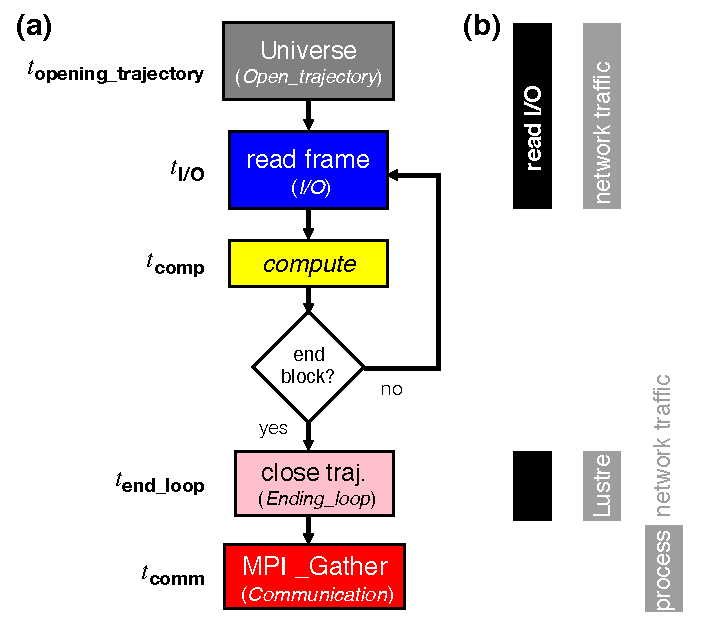
\includegraphics[width=5cm]{figures/flowchart.pdf}
  \caption{Flow chart of the MPI-parallelized RMSD algorithm, Algorithm~\ref{alg:RMSD}.
    Each MPI process performs the same steps but reads trajectory frames from different blocks of the trajectory.
    The color scheme and labels in italics correspond to the colors and labels for measured timing quantitities in the following graphs (e.g., Figs.~\protect\ref{fig:ScalingComputeIO} and \protect\ref{fig:MPIranks}).
    The names of the corresponding timing quantitities from Table \protect\ref{tab:notation} are listed next to each step.
  }
  \label{fig:flowchart}
\end{figure}

As a test case that is representative of a common task in the analysis of biomolecular simulation trajectories we calculated the timeseries of the minimal structural root mean square distance  (\textbf{RMSD}) after rigid body superposition \cite{Lea96, Mura:2014kx}.
The RMSD is used to show the rigidity of protein domains and more generally characterizes structural changes.
It is calculated as a function of time $t$ as
\begin{equation}
  \label{eq:rmsd}
  \text{RMSD}(t) = \min_{\mathsf{R}, \mathbf{t}} %
  \sqrt{\frac{1}{N} \sum_{i=1}^{N} \left[ %
      (\mathsf{R}\cdot\mathbf{x}_{i}(t) + \mathbf{t}) - \mathbf{x}_{i}^{\text{ref}} \right]^{2}}
\end{equation}
where $\mathbf{x}_{i}(t)$ is the position of atom $i$ at time $t$, $\mathbf{x}_{i}^{\text{ref}}$ is its position in a reference structure and the distance between these two is minimized by finding the optimum $3\times3$ rotation matrix $\mathsf{R}$ and translation vector $\mathbf{t}$. 
The optimum rigid body superposition was calculated with the QCPROT algorithm~\cite{Liu:2010kx,Theobald:2005vn} (implemented in Cython and available through the \texttt{MDAnalysis.analysis.rms} module \cite{Gowers:2016aa}).

The RMSD trajectory analysis was parallelized as outlined in the flow chart in Figure~\ref{fig:flowchart}, with further details available in Algorithm~\ref{alg:RMSD}.
Each MPI process loads the core MDAnalysis structure (called the \texttt{Universe}), which includes loading a shared ``topology'' file with the simulation system information and opening the shared trajectory file.
Each process operates on a different block of frames and iterates through them by reading the coordinates of a single frame into memory and performing the RMSD computation with them.
Once all frames in the block are processed, the trajectory file is closed and results are communicated to MPI rank 0 using \texttt{MPI\_Gather()}.

The RMSD was determined for a subset of protein atoms, the $N=214$  C$_{\alpha}$ atoms of our test system (see section \ref{sec:data} for details).
The time complexity for the RMSD Algorithm~\ref{alg:RMSD} is $\mathcal{O}(T \times N^{2})$~\cite{Liu:2010kx} where $T$ is the number of frames in the trajectory and $N$ the number of particles included in the RMSD calculation.

\begin{algorithm}[ht!]
	\scriptsize
	\caption{MPI-parallel Multi-frame RMSD Algorithm}
	\label{alg:RMSD}
	\hspace*{\algorithmicindent} \textbf{Input:} \emph{size}: Total number of frames \\
	\hspace*{\algorithmicindent} \emph{ref}: mobile group in the initial frame which will be considered as reference \\
	\hspace*{\algorithmicindent} \emph{start \& stop}: Starting and stopping frame index\\
	\hspace*{\algorithmicindent} \emph{topology \& trajectory}: files to read the data structure from \\
	\hspace*{\algorithmicindent} \textbf{Output:} Calculated RMSD arrays
	\begin{algorithmic}[1]
		\Procedure{$Block\_RMSD$}{topology, trajectory, $ref$, start, stop}                       
		\State u $\leftarrow$ Universe(topology, trajectory)\Comment{u hold all the information of the physical system}
		\State $g$ $\leftarrow$ u.frames[start:stop]
		\For{$\forall iframe$ in $g$}
		\State $results[iframe] \leftarrow RMSD(g, ref)$
		\EndFor
		\State \Return results
		\EndProcedure
		\\        
		\State MPI Init
		\State rank $\leftarrow$ rank ID
		\State index $\leftarrow$ indices of mobile atom group
		\State xref0 $\leftarrow$ Reference atom group\textsc{\char13}s position
		\State out $\leftarrow$ Block\_RMSD(topology, trajectory, xref0, start=start, stop=stop)
		\\
		\State Gather(out, RMSD\_data, rank\_ID=0)
		\State MPI Finalize
	\end{algorithmic}
\end{algorithm}


\subsection{MPI for Python (\package{mpi4py})}
\label{sec:methods-mpi4py}

MPI for Python (\package{mpi4py}) is a Python wrapper for the Message Passing Interface (MPI) standard and allows any Python program to employ multiple processors \cite{Dalcin:2011aa, Dalcin:2005aa}.
Performance degradation due to using \package{mpi4py} is not prohibitive \cite{Dalcin:2011aa, Dalcin:2005aa} and the overhead is far smaller than the overhead associated with the use of interpreted versus compiled languages \cite{GAiN}.
Overheads in \package{mpi4py} are small compared to C code if efficient raw memory buffers are used for communication \cite{Dalcin:2011aa}, as used in the present study.

\subsection{Global Arrays Toolkit}
\label{sec:methods-ga}

The \emph{Global Arrays} (GA) toolkit provides users with a language interface that allows them to distribute data while maintaining the type of global index space and programming syntax similar to what is available when programming on a single processor \cite{GA}.
It allows manipulating physically distributed dense multi-dimensional arrays without explicitly defining communication and synchronization between processes.
The underlying communication is determined by a runtime environment, which defaults to the \emph{Communication runtime for Extreme Scale} (ComEx) \cite{Daily:2014aa}.
ComEx uses shared memory for intra-node communication and inter-node communication employs ComEx with MPI.
\emph{Global Arrays in NumPy} (GAiN) extends GA to Python through Numpy \cite{GAiN}. 
The \emph{Global Arrays} toolkit provides functions to create global arrays (\texttt{ga\_create()}) and to copy data to (\texttt{ga\_put()}) and from (\texttt{ga\_get()}) such a global array,  as well as additional functions for copying between arrays and freeing them \cite{GAiN}.
When a global array is created (\texttt{ga\_create()}) each process will create an array of the same shape and size, physically located in the local memory space of that process \cite{GA}. 
The GA library maintains a list of all these memory locations, which can be queried with the \texttt{ga\_access()} function.
Using a pointer returned by \texttt{ga\_access()}, one can directly modify the data that is local to each process.
When a process tries to access a block of data the request is first decomposed into individual blocks representing the contribution to the total request from the data held locally on each process (\textit{B. J. Palmer and J. Daily, personal communication}).
The requesting process then makes individual requests to each of the remote processes. 

We investigated if communication cost could be reduced by using \emph{Global Arrays}.
Algorithm \ref{alg:GA} describes the RMSD algorithm with \emph{Global Arrays} instead of MPI.

\begin{algorithm}[ht!]
	\scriptsize
	\caption{MPI-parallel Multi-frame RMSD using Global Arrays}
	\label{alg:GA}
	\hspace*{\algorithmicindent} \textbf{Input:}\emph{size}: Total number of frames assigned to each rank $N_{b}$\\
	\hspace*{\algorithmicindent} \emph{g\_a}: Initialized Global Arrays \\
	\hspace*{\algorithmicindent} \emph{xref0}: mobile group in the initial frame which will be considered as reference \\
	\hspace*{\algorithmicindent} \emph{start \& stop}: that tell which block of trajectory (frames) is assigned to each rank \\
	\hspace*{\algorithmicindent} \emph{topology \& trajectory}: files to read the data structure from \\
	\hspace*{\algorithmicindent}\textbf{Include:} \texttt{Block\_RMSD()} from Algorithm \ref{alg:RMSD}
	\begin{algorithmic}[1]
		
		\State bsize $\leftarrow$ ceil(trajectory.number\_frames / size)
		\State g\_a $\leftarrow$ ga.create(ga.C\_DBL, [bsize*size,2], "RMSD")
		\State buf $\leftarrow$ np.zeros([bsize*size,2], dtype=float)
		\State out $\leftarrow$ Block\_RMSD(topology, trajectory, xref0, start=start, stop=stop)
		\State ga.put(g\_a, out, (start,0), (stop,2))
		\If{rank == 0}
		\State buf $\leftarrow$ ga.get(g\_a, lo=None, hi=None)
		\EndIf
	\end{algorithmic}
\end{algorithm}

\subsection{MPI and Parallel HDF5}
\label{sec:methods-hdf5}

HDF5 is a structured self-describing hierarchical data format which is the standard mechanism for storing large quantities of numerical data in Python (\url{http://www.hdfgroup.org/HDF5}, \cite{pythonhdf5}).
Parallel HDF5 (\package{PHDF5}) typically sits on top of a MPI-IO layer and can use MPI-IO optimizations. 
In \package{PHDF5}, all file access is coordinated by the MPI library; otherwise, multiple processes would compete over accessing the same file on disk. 
MPI-based applications launch multiple parallel instances of the Python interpreter that communicate with each other via the MPI library. 
Implementation is straightforward as long as the user supplies a MPI communicator and takes into account some constraints required for data consistency \cite{pythonhdf5}.
\package{HDF5} itself handles nearly all the details involved with coordinating file access when the shared file is opened through the \emph{mpio} driver.

MPI has two flavors of operation: collective (all processes have to participate in the same order) and independent (processes can perform the operation in any order or not at all) \cite{pythonhdf5}.
With \package{PHDF5}, modifications to file metadata must be performed collectively and although all processes perform the same task, they do not wait until the others catch up \cite{pythonhdf5}. 
Other tasks and any type of data operations can be performed independently by processes.
In the present study, we use independent operations.


\section{Benchmark Environment}
% -*- mode: latex; mode: visual-line; fill-column: 9999; coding: utf-8 -*-

\section{Benchmark Environment}
\label{sec:system}
Our benchmark environment consisted of three different XSEDE \cite{xsede} HPC resources (described in section~\ref{sec:hpcresources}), the software stack used (section~\ref{sec:software}), which had to be compiled for each resource, and the common test data set (section~\ref{sec:data}).

\subsection{HPC Resources}
\label{sec:hpcresources}

The computational experiments were executed on standard compute nodes of three XSEDE \cite{xsede} supercomputers, \emph{SDSC Comet}, \emph{PSC Bridges}, and \emph{LSU SuperMIC} (Table~\ref{tab:sys-config}).
\emph{SDSC Comet} is a 2 PFlop/s cluster with 2,020 compute nodes in total. It is optimized for running a large number of medium-size calculations (up to 1,024 cores) to support the most prevalent type of calculation on XSEDE resources.
\emph{PSC Bridges} is a 1.35 PFlop/s cluster with different types of computational nodes, including 16 GPU nodes, 8 large memory and 2 extreme memory nodes, and 752 regular nodes.
It was designed to flexibly support both traditional (medium scale calculations) and non-traditional (data analytics) HPC uses.
\emph{LSU SuperMIC} offers 360 standard compute nodes with a peak performance of 557 TFlop/s.
The parallel file system on all three machines is Lustre (\url{http://lustre.org/}) and is shared between the nodes of each cluster.

\begin{table}[ht!]
        \centering
  	\caption[Configuration of HPC resources]
	{Configuration of the HPC resources that were benchmarked. Only a subset of the total available nodes were used. IB: InfiniBand; OPA: Omni-Path Architecture.}
	\label{tab:sys-config}
	\begin{adjustbox}{max width=\textwidth}
		\begin{tabular}{c c c c c c c c c}
			\toprule
			\bfseries\thead{Name} & \bfseries\thead{Nodes} & \makecell{\bfseries\thead{Number \\of Nodes}} & \bfseries\thead{CPUs} &  \bfseries\thead{RAM} & \bfseries\thead{Network Topology} & \makecell{\bfseries\thead{Scheduler and  \\ Resource Manager}} & \makecell{\bfseries\thead{parallel\\file system}}\\
			\midrule
			\bfseries \emph{SDSC Comet} & Compute & 6400 & \makecell{2 Intel Xeon (E5-2680v3) \\ 12 cores/CPU, 2.5 GHz} &128 GB DDR4 DRAM & 56 Gbps IB & SLURM & Lustre\\
			\bfseries \emph{PSC Bridges} & RSM & 752 & \makecell{2 Intel Haswell (E5-2695 v3)  \\14 cores/CPU, 2.3 GHz} & 128 GB, DDR4-2133MHz & 12.37 Gbps OPA & SLURM & Lustre\\
			\bfseries \emph{LSU SuperMIC} & Standard & 360 & \makecell{2 Intel Ivy Bridge (E5-2680) \\10 cores/CPU, 2.8 GHz} & 64 GB, DDR3-1866MHz  & 56 Gbps IB & PBS & Lustre\\
			\bottomrule
		\end{tabular}
	\end{adjustbox}
\end{table}

\subsection{Software}
\label{sec:software}

Table~\ref{tab:version} lists the tools and libraries that were required for our computational experiments.  Many domain specific packages are not available in the standard software installation on supercomputers.
We therefore had to compile them, which in some cases required substantial effort due to non-standard building and installation procedures or lack of good documentation.
Because this is a common problem that hinders reproducibility we provide detailed version information, notes on the installation process, as well as comments on the ease of installation and the quality of the documentation in Table~\ref{tab:version}.
For the MPI implementation we used Open MPI release 1.10.7  (\url{https://www.open-mpi.org/}) consistently everywhere.
We used the \package{h5py} package for HDF5, which enables parallel HDF5 from Python because its dependencies, the HDF5 library itself and \package{mpi4py}, were both built against Open MPI.
We used Python 2.7 because it provided maximum compatibility between packages at the time when the project was started.
However, since January 2020, Python 2.7 is officially unsupported.
In principle the complete Python-dependent software stack could also be set up with Python 3.5 or higher, except package \package{ga4py}, which is no longer maintained and remains only available under Python 2.7 (\url{https://github.com/GlobalArrays/ga4py/issues/2}).
Detailed instructions to create the computing environments together with the benchmarking code can be found in the GitHub repository as described in Section~\ref{sec:sharing}.
Carefully setting up the same software stack on the three different supercomputers allowed us to clearly demonstrate the reproducibility of our results and showed that our findings were not dependent on machine specifics.


\begin{table}[ht!]
\centering
\caption[Version of the packages used in the present study]%
{Detailed comparison on the dependencies and installation of different software packages used in the present study. Software was built from source or obtained via a package manager and installed on the multi-user HPC systems in Table~\protect\ref{tab:sys-config}. Evaluation of ease of installation and documentation uses a subjective scale with ``++'' (excellent), ``+'' (good), ``0'' (average), and ``$-$'' (difficult/lacking) and reflects the experience of a typical domain scientist at the graduate/post-graduate level in a discipline such as computational biophysics or chemistry.}
\label{tab:version}  
\begin{adjustbox}{max width=\textwidth}
\begin{tabular}{l c l c c l l}
  \toprule
            \bfseries\thead{Package} & \bfseries\thead{Version} & \bfseries\thead{Description} & \bfseries\thead{Ease of Installation} & \bfseries\thead{Documentation} & \bfseries\thead{Installation} & \bfseries\thead{Dependencies}\\
  \midrule
   \bfseries GCC & 4.9.4 & GNU Compiler Collection & 0 & ++ & \makecell[l]{via configuration \\files, environment \\or command line options, \\ minimal configuration \\ is required} &--\\
   \midrule
   \bfseries Open MPI & 1.10.7 & MPI Implementation & 0 & ++ & \makecell[l]{via configuration \\ files, environment \\or command line options, \\ minimal configuration \\ is required} &--\\
   \midrule
   \bfseries Global Arrays & 5.6.1 & Global Arrays & $-$ & + & \makecell[l]{via configuration files, \\ environment \\or command line options, \\ several optional configuration\\ settings available} & \makecell[l]{MAMA, ARMCI\\ MPI 1.x/2.x/3.x \\ implementation like \\ Open MPI \\ built with shared/dynamic\\ libraries, GCC}\\
   \midrule
   \bfseries Python & 2.7.13 & Python language & + & ++ & Conda Installation & --\\
   \midrule
   \bfseries mpi4py & 3.0.0 & MPI for Python & + & ++ & Conda Installation &\makecell[l]{Python 2.7 or above, \\ MPI 1.x/2.x/3.x  \\ implementation like \\ Open MPI \\built with shared/dynamic \\libraries, Cython}\\
   \midrule
   \bfseries GA4py & 1.0 & Global Arrays for Python & 0 & 0 & Python setuptools &\makecell[l]{Global Arrays, Python 2 only,\\ MPI 1.x/2.x/3.x  \\implementation like \\ Open MPI \\ built with shared/dynamic \\libraries, Cython,  \\mpi4py, Numpy} \\
   \midrule
   \bfseries PHDF5 & 1.10.1 & Parallel HDF5 & $-$ & ++ & \makecell[l]{via configuration files,\\ environment \\or command line options, \\ several optional configuration\\ settings available} &\makecell[l]{MPI 1.x/2.x/3.x  \\ implementation like \\ Open MPI  \\GNU, MPIF90,  \\MPICC, MPICXX}\\
   \midrule
   \bfseries h5py &  2.7.1 & Pythonic wrapper around the HDF5 & + & ++ & Conda Installation & \makecell[l]{Python 2.7, or above,\\ PHDF5, Cython}\\    
   \midrule
   \bfseries MDAnalysis & 0.17.0 & \makecell[l]{Python library to analyze \\trajectories from MD simulations} & + & ++ & Conda Installation & \makecell[l]{Python $>=$2.7, Cython,\\ GNU, Numpy}\\
  \bottomrule
\end{tabular}
\end{adjustbox}
\end{table}


\subsection{Data Set}
\label{sec:data}

The test system contained the protein adenylate kinase with 214 amino acid residues and 3341 atoms in total~\cite{Seyler:2014il} and the topology information (atoms types and bonds) was stored in a file in CHARMM PSF format.
The test trajectory was created by concatenating 600 copies of a MD trajectory with 4,187 time frames (saved every 240~ps for a total simulated time of 1.004~$\mu\text{s}$) in CHARMM DCD format~\cite{Seyler:2017aa} and converting to Gromacs XTC format trajectory, as described for the ``600x'' trajectory in~\citet{Khoshlessan:2017ab}.
The trajectory had a file size of about 30 GB and contained 2,512,200 frames (corresponding to 602.4~$\mu\text{s}$ simulated time).
The file size was relatively small because water molecules that were also part of the original MD simulations were stripped to reduce the original file size by a factor of about 10; such preprocessing is a common approach if one is only interested in the protein behavior.
Thus, the trajectory represents a small to medium system size in the number of atoms and coordinates that have to be loaded into memory for each time frame.
The XTC format is a format with lossy compression \cite{Lindahl01, Spangberg:2011zr}, which also contributed to the compact file size.
XTC trades lower I/O demands for higher CPU demands during decompression and therefore performed well in our previous study~\cite{Khoshlessan:2017ab}.
In order to assess the performance of reading from an HDF5 file in parallel (see Section~\ref{sec:methods-hdf5}) we generated a trajectory-like HDF5 file with the data required to perform the RMSD calculation.
This HDF5 file was created from the XTC file by sub-selecting the atoms for which the RMSD was calculated as detailed in Section~\ref{sec:mda}; a Python script to perform the trajectory conversion can be found in the GitHub repository (see Section~\ref{sec:sharing}).
The coordinates were stored as a two-dimensional $T \times 3N$ array where the first dimension contained $T=2,512,200$ frames and the second dimension the $3N = 438$ Cartesian coordinates.
Although 2,512,200 frames represents a long simulation for current standards, such trajectories will become increasingly common due to the use of special hardware~\cite{Shaw:2009ly, Shaw:2014aa} and GPU-acceleration~\cite{Salomon-Ferrer:2013cr, Glaser:2015ys, Abraham:2015aa}.



\section{Methods}
\label{sec:methods}

Documentation and benchmark codes are made available in the code repository \url{https://github.com/hpcanalytics/supplement-hpc-py-parallel-mdanalysis} under the GNU General Public License v3.0 (code) and the Creative Commons Attribution-ShareAlike (documentation). 
These materials should enable users to recreate the computational environment on the tested XSEDE HPC resources (\emph{SDSC Comet}, \emph{PSC Bridges}, \emph{LSU SuperMIC}), prepare data files, and run the computational experiments.

In the following we define the quantities and approach used for our performance measurements, with a full summary of all definitions in Table~\ref{tab:notation}.
We evaluated MPI performance of the parallel RMSD timeseries algorithm~\ref{alg:RMSD} by timing the total time to solution as well as the execution time for different parts of the code for individual MPI ranks with the help of the Python \texttt{time.time()} function.


\begin{table}
\centering
\begin{tabular}{c c}
  \toprule
           \bfseries\thead{Quantity} & \bfseries\thead{Definition}\\
  \midrule
    $N_{\text{b}}$ & $N_{\text{frames}}^{\text{total}}/N$\\  
    $t_{\text{end\_loop}}$ & $t_{\text{L6}}+t_{\text{L7}}$\\
    $t_{\text{opening\_trajectory}}$ &  $t_{\text{L2}}+t_{\text{L3}}$ \\
    $\tcomp$ & $\sum_{\text{frame}=1}^{N_{\text{b}}}\tcomp^{\text{frame}}$\\
    $\tIO$ & $\sum_{\text{frame}=1}^{N_{\text{b}}}\tIO^{\text{frame}}$\\
    $t_{\text{all\_frame}}$ & $t_{\text{L4}}+t_{\text{L5}}+t_{\text{L6}}$  \\
    $t_{\text{RMSD}}$ &  $t_{\text{L1}} + ...+ t_{\text{L8}}$ \\
    $t_{\text{comm/MPI}}$ &  $t_{\text{L16}}$  \\
    $t_{\text{comm/GA}}$ &  $t_{\text{L5}}+t_{\text{L6}}+t_{\text{L7}}+t_{\text{L8}}$  \\
    $\tcomm$  & $t_{\text{comm/MPI}}$ (Alg.~\ref{alg:RMSD}) or $t_{\text{comm/GA}}$ (Alg.~\ref{alg:GA})\\
    $t_{\text{Overhead1}}$ & $t_{\text{all\_frame}}-t_{\text{I/O\_final}}-t_{\text{comp\_final}}-t_{\text{end\_loop}}$  \\
    $t_{\text{Overhead2}}$ & $t_{\text{RMSD}}-t_{\text{all\_frame}}-t_{\text{opening\_trajectory}}$  \\
    $t_{N}$ & $t_{\text{RMSD}}+\tcomm$ \\
   \midrule  
    $\overline{\tcomp}$ & $\frac{1}{N}\sum_{\text{rank}=1}^{N} \tcomp$ \\
    $\overline{\tIO}$ & $\frac{1}{N}\sum_{\text{rank}=1}^{N} \tIO$\\
    $\overline{\tcomm}$ & $\frac{1}{N}\sum_{\text{rank}=1}^{N} \tcomm$ \\
    $t_{\text{total}}$ & $\max t_{N}$ \\
  \bottomrule
\end{tabular}
\caption[Summary of the notation of our performance modeling]
{Summary of measured timing quantitities.
Timings are collected for the specified line numbers in the code, labelled as $t_{\text{L$n$}}$ where $\text{L$n$}$ refers to the line number in the corresponding algorithm. 
$t_{\text{comm/MPI}}$ (in Algorithm~\protect\ref{alg:RMSD})and $t_{\text{comm/GA}}$ (in Algorithm~\protect\ref{alg:GA}) are both referred to as $\tcomm$ in the text.
$t_{\text{I/O\_final}}$ and $t_{\text{comp\_final}}$ are the timings of the last frame in the block of frames that is processed by the MPI rank and are subtracted to avoid double counting.
Variables in the top half of the table refer to measurements of an individual MPI rank.
Variables in the bottom half are aggregates such as averages over all ranks or the total time to solution.}
\label{tab:notation}
\end{table}


\subsection{Timing observables}

We abbreviate the timings in the following as variables $t_{\text{L$n$}}$ where $\text{L$n$}$ refers to the line number in algorithm~\ref{alg:RMSD}.
We measured in the function \texttt{block\_rmsd()} the \emph{read I/O time} for ingesting the data of one trajectory frame from the file system into memory, $t_{\text{I/O}}^{\text{frame}} = t_{\text{L4}}$, and the \emph{compute time} per trajectory frame to perform the computation, $\tcomp^{\text{frame}} = t_{\text{L5}}$.
The \emph{total read I/O time for a MPI rank},  $\tIO = \sum_{\text{frame}=1}^{N_{\text{b}}} \tIO^{\text{frame}}$, is the sum over all I/O times for all the $N_{\text{frames}}$ frames assigned to the rank; similarly, the \emph{total compute time for a MPI rank} is $\tcomp = \sum_{\text{frame}=1}^{N_{\text{b}}} \tcomp^{\text{frame}}$. 
The time delay between the end of the last iteration and exiting the \texttt{for} loop is $t_{\text{end\_loop}} = t_{\text{L6}}+t_{\text{L7}}$.
The time $t_{\text{opening\_trajectory}} = t_{\text{L2}}+t_{\text{L3}}$ measures the problem setup, which includes data structure initialization and opening of topology and trajectory files.
The \emph{communication time}, $\tcomm = t_{\text{L16}}$, is the time to gather all data from all processor ranks to rank zero.
The total time (for all frames) spent in \texttt{block\_rmsd()} is $t_{\text{RMSD}} = \sum_{i=1}^{8}t_{\text{L$i$}}$. 
There are parts of the code in \texttt{block\_rmsd()} that are not covered by the detailed timing information of \tcomp and \tIO.
Unaccounted time is considered as \emph{overhead}.
We define $t_{\text{Overhead1}}$ and $t_{\text{Overhead2}}$ as the overheads of the calculations (see Table \ref{tab:notation} for the definitions); both should ideally be negligible. 
Finally, the \emph{total time to completion of a single MPI rank}, when utilizing $N$ cores for the execution of the overall experiment, is $t_{N}$, and as a result $t_{\text{RMSD}} + \tcomm \equiv t_{N}$.

\subsection{Performance parameters}

We measured the \emph{total time to solution} $t_{\text{total}}(N)$ with $N$ MPI processes on $N$ cores, which is effectively
$t_{\text{total}}(N) \approx \max(t_{N})$. 
Strong scaling was quantified by the speed-up
\begin{equation}
  \label{eq:speedup}
  S(N) = \frac{t_{\text{total}}(N)}{t_{\text{total}}(1)},
\end{equation}
relative to performance on a single core, and the efficiency
\begin{equation}
  \label{eq:efficiency}
  E(N) = \frac{S(N)}{N}.
\end{equation}
Averages over ranks were calculated as
\begin{equation}
  \label{eq:avg-tcomp}
  \overline{\tcomp} = \frac{1}{N}
  \sum_{\text{rank}=1}^{N}\tcomp = \frac{1}{N}\sum_{\text{rank}=1}^{N}\sum_{\text{frame}=1}^{N_\text{b}}\tcomp^{\text{frame}},
\end{equation}
\begin{equation}
  \label{eq:avg-tIO}
  \overline{\tIO} = \frac{1}{N}\sum_{\text{rank}=1}^{N}\tIO = \frac{1}{N}\sum_{\text{rank}=1}^{N}\sum_{\text{frame}=1}^{N_{\text{b}}}\tIO^{\text{frame}},
\end{equation}
and
\begin{equation}
  \label{eq:avg-tcomm}
  \overline{\tcomm} = \frac{1}{N}\sum_{\text{rank}=1}^{N}\tcomm.
\end{equation}

Additionally, we introduced two performance parameters that will be shown to be indicative of the occurrence of stragglers.
We defined the ratio of compute time to read I/O time as
\begin{equation}
  \RcompIO = \frac{\tcomp}{\tIO}.
  \label{eq:Compute-IO}
\end{equation}
\RcompIO was calculated with the serial version of our algorithms (on a single CPU core) in order to characterize the computational problem in the absence of parallelization.
The ratio of compute to communication time was defined by the ratio of average total compute time per rank to the average total communication time per rank  
\begin{equation}
  \label{eq:Compute-comm}
  \Rcompcomm = \frac{\overline{\tcomp}}{\overline{\tcomm}}.
\end{equation}
Because \tcomm cannot be measured for a serial code, we estimated \Rcompcomm from the rank-averages (Eqs.~\ref{eq:avg-tcomp} and \ref{eq:avg-tcomm}) for a given number of MPI ranks.


\section{Computational Experiments}
% -*- mode: latex; mode: visual-line; fill-column: 9999; coding: utf-8 -*-

\section{Computational Experiments}
\label{sec:experiments}

We had previously measured the performance of the MPI-parallelized RMSD analysis task on two different HPC resources (\emph{SDSC Comet} and \emph{TACC Stampede}) and had found that it only scaled well up to a single node due to high variance in the runtime of the MPI ranks, similar to the straggler phenomenon observed in big-data analytics \cite{Khoshlessan:2017ab}.
However, the ultimate cause for this high variance could not be ascertained.
We therefore performed more measurements with more detailed timing information (see section \ref{sec:methods}) on \emph{SDSC Comet} (described in this section) and two other supercomputers (summarized in section \ref{sec:clusters}) in order to better understand the origin of the stragglers and find solutions to overcome them. 

\subsection{RMSD Benchmark}
\label{sec:RMSD}

We measured strong scaling for the RMSD analysis task (Algorithm \ref{alg:RMSD}) with the 2,512,200 frame test trajectory (section \ref{sec:data}) on 1 to 72 cores (one to three nodes) of \emph{SDSC Comet} (Figures~\ref{fig:MPIscaling} and \ref{fig:MPIspeedup}). 
We observed poor strong scaling performance beyond a single node (24 cores), comparable to our previous results \cite{Khoshlessan:2017ab}.
A more detailed analysis showed that the RMSD computation, and to a lesser degree the read I/O, considered on their own, scaled well beyond 50 cores (yellow and blue lines in Figure~\ref{fig:ScalingComputeIO}). 
But communication (sending results back to MPI rank 0 with \texttt{MPI\_Gather()}; red line in Figure~\ref{fig:ScalingComputeIO}) and the initial file opening (loading the system information into the \texttt{MDAnalysis.Universe} data structure from a shared topology file and opening the shared trajectory file; gray line in Figure~\ref{fig:ScalingComputeIO}) started to dominate beyond 50 cores.
Communication cost and initial time for opening the trajectory were distributed unevenly across MPI ranks, as shown in Figure~\ref{fig:MPIranks}. 
The ranks that took much longer to complete than the typical execution time of the other ranks were the stragglers that hurt performance.

\begin{figure}[!htb]
  \centering
  \begin{subfigure}{.4\textwidth}
    \includegraphics[width=\linewidth]{figures/main-RMSD-t_total.pdf}
    \captionsetup{format=hang}
    \caption{Scaling total (five repeats)}
    \label{fig:MPIscaling}
  \end{subfigure}
  \hfill
  \begin{subfigure}{.4\textwidth}
    \includegraphics[width=\linewidth]{figures/main-RMSD-speed_up.pdf}
    \captionsetup{format=hang}
    \caption{Speed-up (five repeats)}
    \label{fig:MPIspeedup}
  \end{subfigure}
  \bigskip
  \begin{subfigure}{.45\textwidth}
    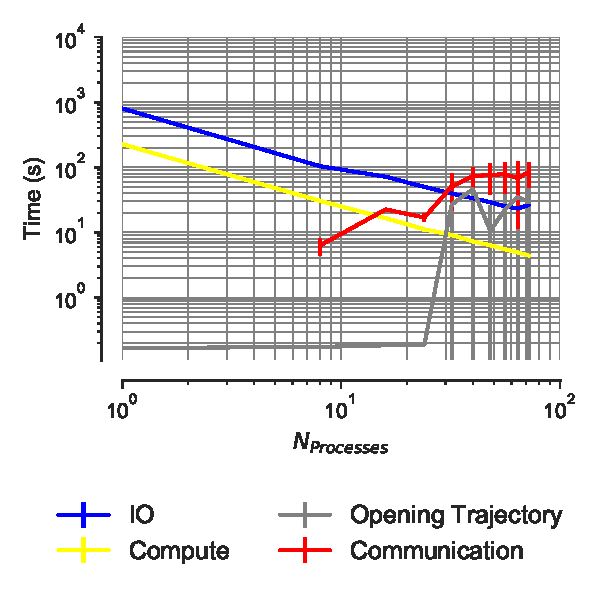
\includegraphics[width=\linewidth]{figures/main-RMSD-time_comp_IO_comparison.pdf}
    \captionsetup{format=hang}
    \caption{Scaling for different components (five repeats)}
    \label{fig:ScalingComputeIO}
  \end{subfigure}
  \hfill
  \begin{subfigure} {.5\textwidth}
    \includegraphics[width=\linewidth]{figures/main-RMSD-BarPlot-rank-comparison_72_5.pdf}
    \captionsetup{format=hang}
    \caption{Time comparison on different parts of the calculations per MPI rank (example)}
    \label{fig:MPIranks}
  \end{subfigure}
  \caption{Performance of the RMSD task parallelized with MPI on \emph{SDSC Comet}.
    Results were communicated back to rank 0.
    Five independent repeats were performed to collect statistics.
    (a-c) The error bars show standard deviation with respect to the mean.
    In serial, there is no communication and no data points are shown for $N=1$ in (c).
    (d) Compute \tcomp, read I/O \tIO, communication \tcomm, ending the for loop $t_{\text{end\_loop}}$, opening the trajectory $t_{\text{opening\_trajectory}}$, and overheads $t_{\text{overhead1}}$, $t_{\text{overhead2}}$ per MPI rank; see Table \ref{tab:notation} for definitions.
    These are data from one run of the five repeats.
    MPI ranks 0, 12--27 and 29--72 are stragglers.
  }
  \label{fig:MPIwithIO}
\end{figure}

We qualitatively denoted by \emph{straggler} any MPI rank that took at least about twice as long as the group of ranks that finished fastest, roughly following the original description of a straggler as a task that took an ``unusually long time to complete'' \cite{Dean2008}.
The fast-finishing ranks were generally clearly distinguishable in the per-rank timings such as in Figures~\ref{fig:MPIranks} and \ref{fig:MPIranks-Bridges}.
Such a qualitative definition of stragglers was sufficient for our purpose of identifying scalability bottlenecks, as shown in the following discussion.

\subsubsection*{Identification of Scalability Bottlenecks}

In the example shown in Figure~\ref{fig:MPIranks}, 62 ranks out of 72 took about 60~s (the stragglers) whereas the remaining ranks only took about 20~s.
In other instances, far fewer ranks were stragglers, as shown, for example, in Figure~\ref{fig:MPIranks-Bridges}.
The detailed breakdown of the time spent on each rank (Figure~\ref{fig:MPIranks}) showed that the computation, \tcomp, was relatively constant across ranks. 
The time spent on reading data from the shared trajectory file on the Lustre file system into memory, \tIO, showed variability across different ranks. 
The stragglers, however, appeared to be defined by occasionally much larger \emph{communication} times, \tcomm (line 16 in Algorithm~\ref{alg:RMSD}), which were on the order of 30~s, and by larger times to initially open the trajectory (line 2 in Algorithm~\ref{alg:RMSD}).
\tcomm varied across different ranks and was barely measurable for a few of them.
Although the data in Figure~\ref{fig:MPIranks} represented one run and in other instances different number of ranks were stragglers, the averages over all ranks in five independent repeats (Figure~\ref{fig:ScalingComputeIO}) showed that increased \tcomm were generally the reason for large variations in the run time for each rank.
This initial analysis indicated that communication was a major issue that prevented good scaling beyond a single node but the problems related to file I/O also played an important role in limiting scaling performance.


\subsubsection*{Influence of Hardware}
We ran the same benchmarks on multiple HPC systems that were equipped with a Lustre parallel file system [XSEDE's \emph{PSC Bridges} (Figure~\ref{fig:MPIwithIO-Bridges}) and \emph{LSU SuperMIC} (Figure~\ref{fig:MPIwithIO-SuperMIC})], and observed the occurrence of stragglers, in a manner very similar to the results described for \emph{SDSC Comet}.
There was no clear pattern in which certain MPI ranks would always be a straggler, and neither could we trace stragglers to specific cores or nodes.
Therefore, the phenomenon of stragglers in the RMSD case was reproducible on different clusters and thus appeared to be independent from the underlying hardware.

\subsection{Effect of Compute to I/O Ratio on Performance}
\label{sec:bound}

The results in section~\ref{sec:RMSD} indicated opening the trajectory, communication, and read I/O to be important factors that appeared to correlate with stragglers. 
In order to better characterize the RMSD task, we computed the ratio between the time to complete the computation and the time spent on I/O per frame, \RcompIO (Eq.~\ref{eq:Compute-IO}).
The average values were $\overline{\tcomp^{\text{frame}}} = 0.09\ \text{ms}$, $\overline{t_{\text{IO}}^{\text{frame}}} = 0.3\ \text{ms}$, resulting in a compute-to-I/O ratio $\RcompIO \approx 0.3$.
With $\RcompIO \ll 1$, the RMSD analysis task was characterized as I/O bound.

In other studies, better scaling was observed for analysis tasks that were more compute-intensive than the RMSD calculation, such as a radial distribution function calculation \cite{Roe:2018aa, Fan:2019aa}, i.e., analysis tasks that could be characterized as compute-bound.
Such behavior is expected, as the contribution from the parallel part of the program that requires neither I/O nor communication is increased.
From a practical point of view, it is of interest to understand the size of the effect of increasing the computational load on strong scaling, and in our case, we were interested in seeing if changes in the compute part (namely the RMSD calculation on coordinates held in memory) would have an effect on the execution time of other parts of the program.
In Appendix~\ref{sec:shiftload} we set out to analyze compute bound tasks, i.e.\ ones with $\RcompIO \gg 1$.
To assess the effect of the $\RcompIO$ ratio on performance while leaving other parameters the same, we artificially increased the computational load by repeating the RMSD calculation and measured strong scaling (Figure \ref{fig:tcomp_tIO_effect}).
With increasing $\RcompIO$, the impact of stragglers appeared to lessen (although they did not disappear) and scaling performance improved, as expected (see Appendix \ref{sec:increasedworkload}).
Better scaling also went together with a higher ratio of compute to communication ($\Rcompcomm$, Eq.~\ref{eq:Compute-comm}) as shown in Appendix \ref{sec:tcomm} but ultimately I/O seemed to be the key determinant for performance.

 \begin{figure}[!htb]
   \centering
   \begin{subfigure}{.25\textwidth}
     \includegraphics[width=\linewidth]{figures/speed_up-effect-of-IO.pdf}
     \caption{Speed up comparison}
     \label{fig:MPIspeedup-no-IO}
   \end{subfigure}
   \begin{subfigure}{0.3\textwidth}
     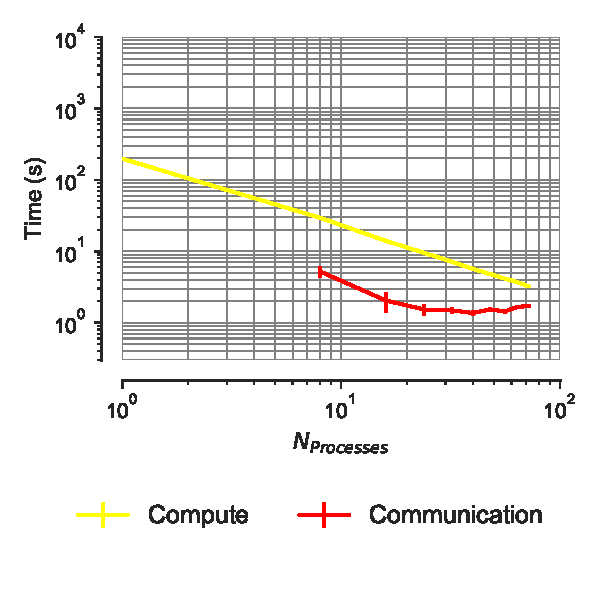
\includegraphics[width=\linewidth]{figures/time_comp_IO_comparison_no-IO.pdf}
     \caption{Scaling for different components}
     \label{fig:MPIScalingCompute-Comm-no-IO}     
   \end{subfigure}
   \begin{subfigure}{.4\textwidth}
     \includegraphics[width=\linewidth]{figures/BarPlot-rank-comparison-no-IO.pdf}
     \captionsetup{format=hang}
     \caption{Time comparison on different parts of the calculations per MPI rank when I/O is removed}
     \label{fig:MPIranks-no-IO}
   \end{subfigure}
   \caption{Comparison of the performance of the RMSD task with I/O ($\RcompIO \approx 0.3$) and without I/O ($\RcompIO = +\infty$) on \emph{SDSC Comet}.
     Five repeats were performed to collect statistics.
     (a-b) The error bars show standard deviation with respect to the mean.
     (b) Only compute \tcomp and communication \tcomm are included; there are no timings related to I/O (\tIO, $t_{\text{opening\_trajectory}}$) as in Figure~\protect{\ref{fig:ScalingComputeIO}}.
     (c) Compute \tcomp, read I/O $\tIO=0$, communication \tcomm, ending the for loop \text{$t_{\text{end\_loop}}$},
     opening the trajectory \text{$t_{\text{opening\_trajectory}}$}, and overheads \text{$t_{\text{overhead1}}$}, \text{$t_{\text{overhead2}}$} per MPI rank.
     (See Table \ref{tab:notation} for definitions.)}
   \label{fig:MPIwithoutIO}
\end{figure}

In order to study an extreme case of a compute-bound task that would demonstrate the effect of ``ideal'' read I/O, we eliminated all I/O from the RMSD task by randomly generating artificial trajectory data in memory; the data had the same size as if they had been obtained from the trajectory file.
The time for the data generation was excluded and no file access was necessary. 
Without any I/O, performance improved markedly (Figure~\ref{fig:MPIwithoutIO}), with reasonable scaling up to 72 cores (3 nodes).
No stragglers were observed because overall communication time decreased dramatically by more than a factor of ten and showed less variability (Figure~\ref{fig:MPIScalingCompute-Comm-no-IO}) compared to the same runs with I/O (Figure~\ref{fig:ScalingComputeIO}), even though exactly the same amount of data were communicated.
The scaling performance suffered somewhat for more than 40 processes only because the cost of communication \tcomm became comparable to the compute time \tcomp and would not decrease further.
Although in practice I/O cannot be avoided, this experiment demonstrated that the way how the trajectory file was accessed on the Lustre file system was at least one cause for the observed stragglers.
It also showed that the communication cost for the \emph{same amount of data transfer} can be dramatically higher in the presence of I/O. 


\subsection{Reducing I/O Cost}
\label{sec:I/O}
In order to improve performance we needed to employ strategies to avoid the competition over file access across different ranks when the $\RcompIO$ ratio was small.
One obvious approach when using the Lustre parallel file system is to increase the number of stripes, i.e., the number of copies of a file that are stored on different object storage targets (OSTs).
But because in our previous work we did not see scaling performance improvement with varying the stripe count \cite{Khoshlessan:2017ab} we decided to just use the system default, i.e., one stripe per file.
Instead we experimented with two different ways for reducing the I/O cost:
\begin{inparaenum}[1)]
	\item splitting the trajectory file into as many segments as the number of processes (subfiling), thus using file-per-process access, and
	\item using the HDF5 file format together with MPI-IO parallel reads instead of the XTC trajectory format.
\end{inparaenum}
We discuss these two approaches and their performance improvements in detail in the following sections.

\subsubsection{Splitting the Trajectories (subfiling)}
\label{sec:splitting-traj}
\emph{Subfiling} is a mechanism previously used for splitting a large multi-dimensional global array to a number of smaller subarrays in which each smaller array is saved in a separate file. Subfiling reduces the file system control overhead by decreasing the number of processes concurrently accessing a shared file~\cite{scalable-IO, scalable-IO1}.
Because subfiling is known to improve performance of parallel shared-file I/O, we investigated splitting our trajectory file into as many trajectory segments as the number of processes.
The trajectory file was split into $N$ segments, one for each process, with each segment having $N_{b}$ frames. 
This way, each process would access its own trajectory segment file without competing for file accesses. 

We ran a benchmark up to 8 nodes (192 cores) and observed rather better scaling behavior with efficiencies above 0.6 (Figure~\ref{fig:MPIscaling-split} and~\ref{fig:MPIspeedup-split}) with the delay time for stragglers reduced from 65~s to about 10~s for 72 processes. 
However, scaling was still far from ideal due to the MPI communication costs. 
Although the delay due to communication was much smaller than compared to parallel RMSD with shared-file I/O [compare Figure~\ref{fig:MPIranks-split} ($\tcomm^{\text{Straggler}} \gg \tcomp+\tIO$) to Figure~\ref{fig:MPIranks} ($\tcomm^{\text{Straggler}} \approx \tcomp+\tIO$)], it was still delaying several processes and resulted in longer job completion times (Figure~\ref{fig:MPIranks-split}). 
These delayed tasks impacted performance so that speed-up remained far from ideal (Figure~\ref{fig:MPIspeedup-split}).

\begin{figure}[!htb]
  \centering
  \begin{subfigure}{.4\textwidth}
    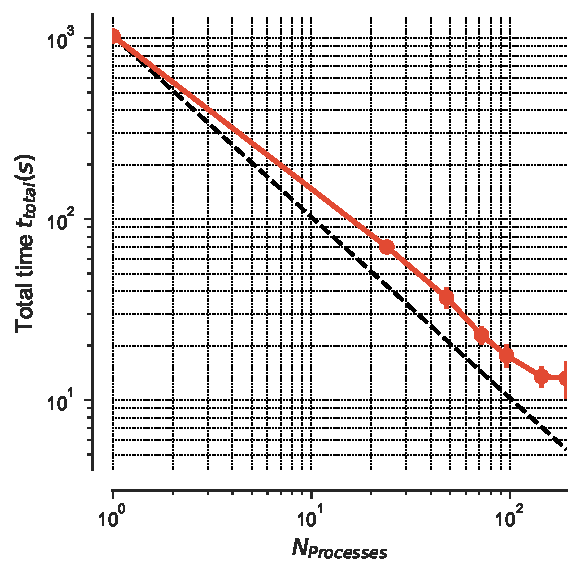
\includegraphics[width=\linewidth]{figures/tot_time_traj_splitting.pdf}
    \caption{Scaling total}
    \label{fig:MPIscaling-split}
  \end{subfigure}
  \hfill
  \begin{subfigure}{.4\textwidth}
    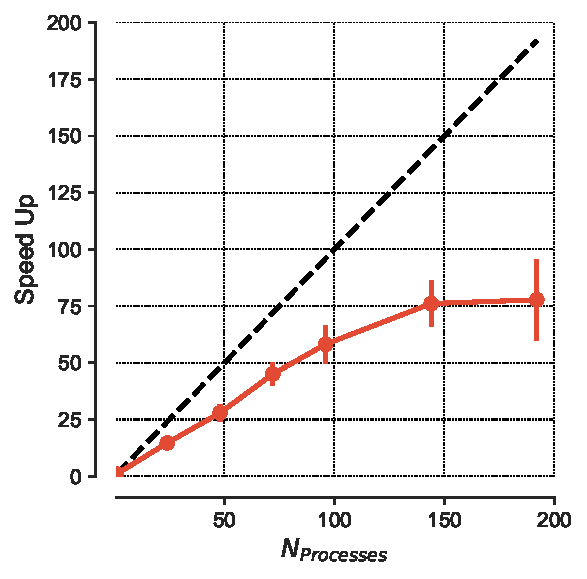
\includegraphics[width=\linewidth]{figures/Speed_UP_traj_splitting.pdf}
    \captionsetup{format=hang}
    \caption{Speed-up}
    \label{fig:MPIspeedup-split}
  \end{subfigure}
  \bigskip
  \begin{subfigure}{.45\textwidth}
    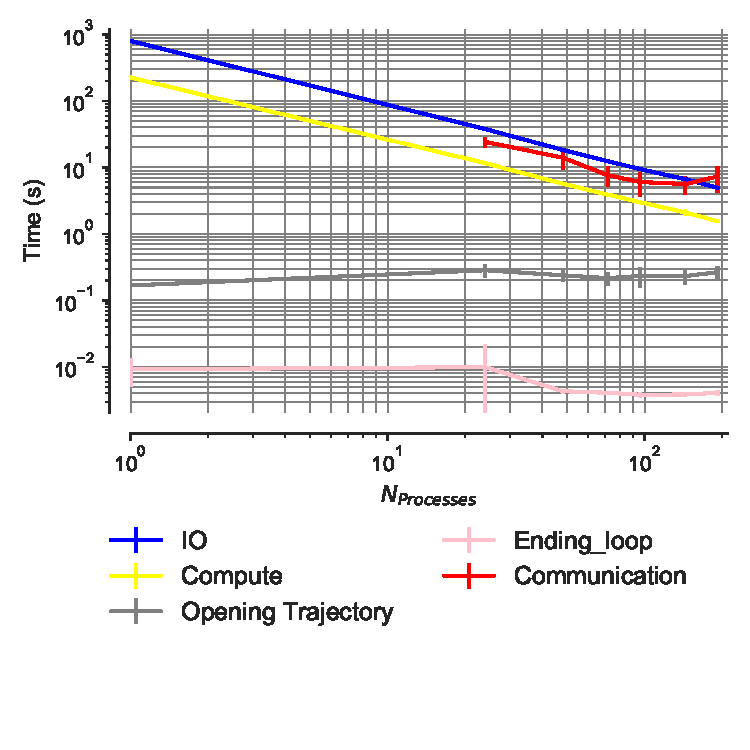
\includegraphics[width=\linewidth]{figures/IO_compute_scaling_traj_splitting.pdf}
    \captionsetup{format=hang}
    \caption{Scaling for different components}
    \label{fig:ScalingComputeIO-split}
  \end{subfigure}
  \hfill
  \begin{subfigure}{.5\textwidth}
    \includegraphics[width=\linewidth]{figures/split-BarPlot-rank-comparison_192_5.pdf}
    \captionsetup{format=hang}
    \caption{Time comparison on different parts of the calculations per MPI rank.}
    \label{fig:MPIranks-split}
  \end{subfigure}
  \caption{Performance of the RMSD task on \emph{SDSC Comet} when the trajectories are split into one trajectory segment per process (\emph{subfiling}).
    Five repeats were performed to collect statistics.
    In serial, there is no communication and no data points are shown for $N=1$ in (c).
    (a-c) The error bars show standard deviation with respect to the mean.
    (d) Compute \tcomp, read I/O \tIO, communication \tcomm, opening the trajectory $t_{\text{opening\_trajectory}}$, ending the for loop  $t_{\text{end\_loop}}$ (includes closing the trajectory), and overheads $t_{\text{overhead1}}$, $t_{\text{overhead2}}$ per MPI rank; see Table \protect\ref{tab:notation} for the definitions.
}
\label{fig:MPIwithIO-split}
\end{figure}


The subfiling approach appeared promising but it required preprocessing of trajectory files and additional storage space for the segments.
We benchmarked the necessary time for splitting the trajectory in parallel using different number of MPI processes (Table~\ref{tab:timing-splitting}); in general the operation scaled well, with efficiencies $> 0.8$ although performance fluctuated, as seen for the case on six nodes where the efficiency dropped to $0.34$ for the run.
These preprocessing times were not included in the estimates because we focused on better understanding the principal causes of stragglers and we wanted to make the results directly comparable to the results of the previous sections.
Nevertheless, from an end user perspective, preprocessing of trajectories can be integrated in workflows (especially as the data in Table~\ref{tab:timing-splitting} indicated good scaling) and the preprocessing time can be quickly amortized if the trajectories are analyzed repeatedly.
However, the requirement of needing as many segments as processes makes the approach somewhat inflexible as a new set of trajectory segments must be produced when a different level of parallelization is needed.
Finally, the performance of parallel file systems generally suffers when too many files are processed and so there exists a limit as to how far the subfiling approach can be pushed.

\begin{SCtable}[1.0][!htb]
  \centering
  \caption[Time necessary for writing the trajectory segments]
  {The wall-clock time spent for writing $N_{\text{seg}}$ trajectory segments using $N_{\text{p}}$ processes using MPI on \emph{SDSC Comet}.
    One set of runs was performed for the timings.
    Scaling $S$ and efficiency $E$ are relative to the 1 node case (24 MPI processes).}
  \label{tab:timing-splitting}  
  \begin{tabular}{rrrrrr}
    \toprule
    \thead{$N_{\text{seg}}$} & \thead{$N_{\text{p}}$} & \thead{nodes}
    & \thead{time (s)} & \thead{$S$} & \thead{$E$}\\
    \midrule
    24 &  24 & 1 & 89.9 & 1.0 & 1.0\\
    48 &  48 & 2 & 46.8 & 1.9 & 0.96\\
    72 &  72 & 3 & 33.7 & 2.7 & 0.89\\
    96 &  96 & 4 & 25.1 & 3.6 & 0.89\\
    144 & 144 & 6 & 43.7 & 2.1 & 0.34\\
    192 & 192 & 8 & 13.5 & 6.7 & 0.83\\  
    \bottomrule
  \end{tabular}
\end{SCtable}


Often trajectories from MD simulations on HPC machines are produced and kept in smaller files or segments that can be concatenated to form a full continuous trajectory file.
These trajectory segments could be used for the subfiling approach.
However, it might not be feasible to have exactly one segment per MPI rank, with all segments of equal size, which constitutes the ideal case for subfiling.
MDAnalysis can create virtual trajectories from separate trajectory segment files that appear to the user as a single trajectory.
In Appendix~\ref{sec:chainreader} we investigated if this so-called \emph{ChainReader} functionality could benefit from the subfiling approach.
We found some improvements in performance but discovered limitations in the design of the ChainReader (namely that all segment files are initially opened) that will have to be addressed before equivalent performance can be reached.
 
\subsubsection{MPI-based Parallel HDF5}
\label{sec:HDF5}

In the HPC community, parallel I/O with MPI-IO is widely used in order to address I/O limitations.
We investigated MPI-based Parallel HDF5 to improve I/O scaling. 
We converted our XTC trajectory file into a simple custom HDF5 format so that we could test the performance of parallel I/O with the HDF5 file format.
The time it took to convert our XTC file with $2,512,200$ frames into HDF5 format was about 5,400~s on a local workstation with network file system (NFS).

\begin{figure}[!htb]
  \centering
  \begin{subfigure}{.4\textwidth}
    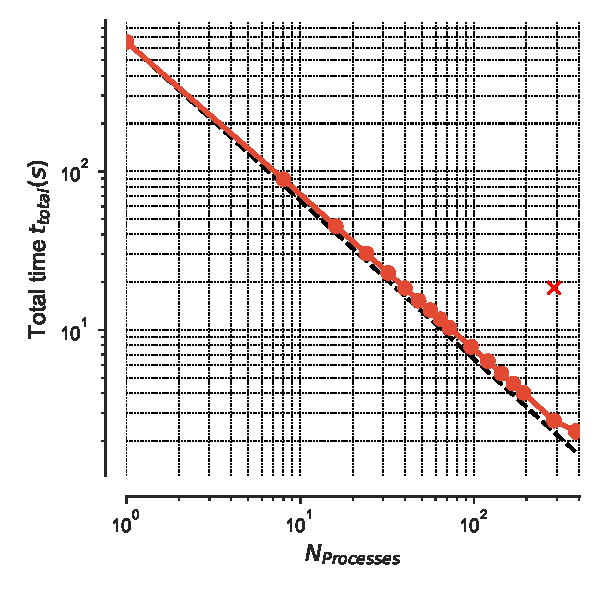
\includegraphics[width=\linewidth]{figures/hdf5-t_total-combined.pdf}
    \caption{Scaling total}
    \label{fig:MPIscaling-hdf5}
  \end{subfigure}
  \hfill
  \begin{subfigure}{.4\textwidth}
    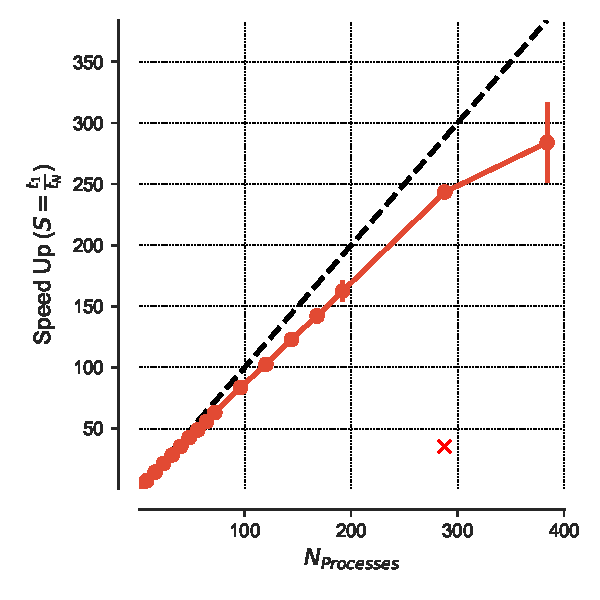
\includegraphics[width=\linewidth]{figures/hdf5-speed_up-combined.pdf}
    \caption{Speed-up}
    \label{fig:MPIspeedup-hdf5}
  \end{subfigure}
  \bigskip

  \begin{subfigure}{.45\textwidth}
    \centering
    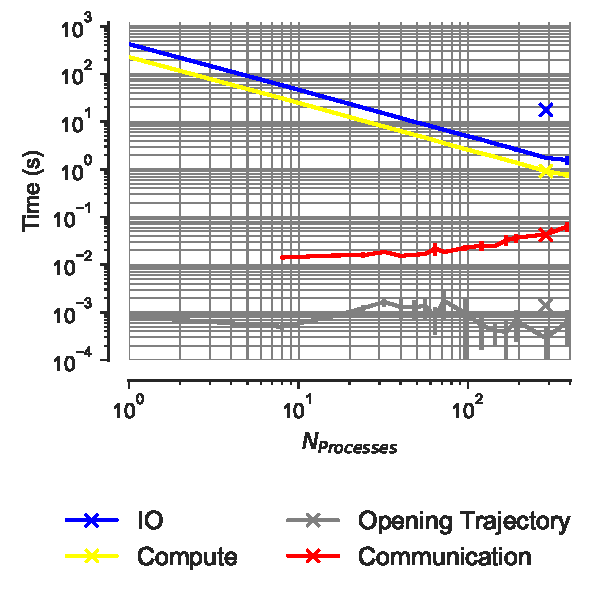
\includegraphics[width=\linewidth]{figures/hdf5-time_comp_IO_comparison-combined.pdf}
    \captionsetup{format=hang}
    \caption{Scaling for different components}
    \label{fig:ScalingComputeIO-hdf5}
  \end{subfigure}
  \hfill
  \begin{subfigure} {.5\textwidth}
    \includegraphics[width=\linewidth]{figures/hdf5-BarPlot-rank-comparison_192_4.pdf}
    \captionsetup{format=hang}
    \caption{Time comparison on different parts of the calculations per MPI rank}
    \label{fig:MPIranks-hdf5}
  \end{subfigure}
  \caption{Performance of the RMSD task with MPI-based parallel HDF5 (MPI-IO) on \emph{SDSC Comet}.
    Data are read from the file system from a shared HDF5 file format instead of XTC format (independent I/O) and results are communicated back to rank 0. 
    Five repeats were performed to collect statistics; one repeat for 288 processes had abnormally high \tIO and was treated as an outlier and excluded from the averages but is shown as ``x'' in the graphs.
    (a-c) The error bars show standard deviation with respect to the mean.
    In serial, there is no communication and no data points are shown for $N=1$ in (c).
    (d) Compute \tcomp, read I/O \tIO, communication \tcomm, ending the for loop $t_{\text{end\_loop}}$,
    opening the trajectory $t_{\text{opening\_trajectory}}$, and overheads $t_{\text{overhead1}}$, $t_{\text{overhead2}}$ per MPI rank; see Table \ref{tab:notation} for definitions.
    These are typical data from one run of the five repeats.
  }
  \label{fig:MPIwithIO-hdf5}
  %  I am reporting the slowest rank per timing, and that is averaged over all repeats.
\end{figure}

We ran our benchmark on up to 16 nodes (384 cores) on \emph{SDSC Comet} and we observed near ideal scaling behavior (Figures~\ref{fig:MPIscaling-hdf5} and~\ref{fig:MPIspeedup-hdf5}) with parallel efficiencies above 0.8 on up to 8 nodes (Figure~\ref{fig:comparison_efficiency}) with no straggler tasks (Figure~\ref{fig:MPIranks-hdf5}).
The trajectory reading I/O (\tIO) was the dominant contribution, followed by compute (\tcomp), but because both contributions scaled well, overall scaling performance remained good, even for 384 cores.
Amongst the five repeats for 12 nodes (288 cores) we observed one run with much slower I/O than typical (Figure~\ref{fig:ScalingComputeIO-hdf5}) but we did not further investigate this spurious case and classified it as an outlier that was excluded from the statistics.
Importantly, the trajectory opening cost remained negligible (in the millisecond range) and the cost for MPI communication also remained small (below 0.1 s, even for 16 nodes).
Overall, parallel MPI with HDF5 appeared to be a robust approach to obtain good scaling, even for I/O-bound tasks.



\subsection{Potential Causes of Stragglers}
\label{sec:likelycauses}

The data indicated that an increase in the duration of both MPI communication and trajectory file access lead to large variability in the run time of individual MPI processes and ultimately poor scaling performance beyond a single node.
A discussion of likely causes for stragglers begins with the observation that opening and reading a single trajectory file from multiple MPI processes appeared to be at the center of the problem. 

In MDAnalysis, individual trajectory frames are loaded into memory, which ensures that even systems with tens of millions of atoms can be efficiently analyzed on resources with moderate RAM sizes.
The test trajectory (file size 30 GB) had $2,512,200$ frames in total so each frame was about 0.011 MB in size.
With $\tIO \approx 0.3~\text{ms}$ per frame, the data were ingested at a rate of about $40$~MB/s for a single process.
For 24 MPI ranks (one \emph{SDSC Comet} node), the aggregated reading rate would have been about 1 GB/s, well within the available bandwidth of 56 Gb/s of the InfiniBand network interface that served the Lustre file system, but nevertheless sufficient to produce substantial constant network traffic.

Furthermore, in our study the default Lustre stripe size value was 1~MB, i.e., the amount of contiguous data stored on a single Lustre OST.
Each I/O request read a single Lustre stripe but because the I/O size (0.011~MB) was smaller than the stripe size, many of these I/O requests were likely just accessing the same stripe on the same OST but nevertheless had to acquire a new reading lock for each request.
The reason for this behavior is related to ensuring POSIX consistency that relates to POSIX I/O API and POSIX I/O semantics, which can have adverse effects on scalability and performance.
Parallel file systems like Lustre implement sophisticated distributed locking mechanisms to ensure consistency.
For example, locking mechanisms ensures that a node can not read from a file or part of a file while it might be being modified by another node. 
When the application I/O is not designed in a way to avoid scenarios where multiple nodes are fighting over locks for overlapping extents, Lustre can suffer from scalability limitations~\cite{optimize_lustre}.
Continuously keeping metadata updated in order to have fully consistent reads and writes (POSIX metadata management), requires writing a new value for the file's last-accessed time (POSIX atime) every time a file is read, imposing a significant burden on parallel file system~\cite{POSIX2017}. 
Mache \textit{et al.} observed that contention for the interconnect between OSTs and compute nodes due to MPI communication may lead to variable performance in I/O measurements~\cite{Mache:2005aa}.
Conversely, our data suggest that single-shared-file I/O on Lustre can negatively affect MPI communication as well, even at moderate numbers (tens to hundreds) of concurrent requests, similar to the results from recent network simulations that predicted interference between MPI and I/O traffic~\cite{Brown:2018ab}.
Brown \textit{et al.}'s  work \cite{Brown:2018ab} indicated that MPI traffic (inter-process communication) could be affected by increasing I/O.
In particular, a few MPI processes were always delayed by one to two orders of magnitude more than the median time, which we would classify as stragglers.
In summary, our observations, seen in the context of the work by \citet{Brown:2018ab}, suggest that our observed stragglers with large variance in the communication step could be due to interference of MPI communications with the I/O requests on the same network.
Further detailed work will be needed to test this hypothesis.

Our results clearly showed that reading a single shared file is an inefficient way to use the Lustre parallel file system; instead, parallel I/O via MPI-IO and HDF5 emerged as the most promising approach to avoid stragglers and obtain good strong scaling behavior on hundreds of cores, even for I/O bound analysis tasks.



\section{Reproducibility and Performance Comparison on Different Clusters}
% -*- mode: latex; mode: visual-line; fill-column: 9999; coding: utf-8 -*-

\section{Reproducibility and Performance Comparison on Different Clusters}
\label{sec:clusters}

In this section we compare the performance of the RMSD task on different HPC resources (Table \ref{tab:sys-config}) to examine the robustness of the methods we used for our performance study and to ensure that the results are general and independent from the specific HPC system.
Scripts and instructions to set up the computational environments and reproduce our computational experiments are provided in a git repository as described in section \ref{sec:methods}.

In \ref{sec:supplement}, we demonstrated that stragglers occur on \emph{PSC Bridges} (Figure \ref{fig:MPIwithIO-Bridges}) and \emph{LSU SuperMIC} (Figure \ref{fig:MPIwithIO-SuperMIC}) in a manner similar to the one observed on \emph{SDSC Comet} (section \ref{sec:RMSD}).
We performed additional comparisons for several cases discussed previously, namely (1) splitting the trajectories with blocking collective communications in MPI, (2) splitting the trajectories with Global Arrays for communications, and (3) MPI-based parallel HDF5.

\subsection{Splitting the Trajectories}
Figure \ref{fig:MPI-splitting-clusters} shows the strong scaling of the RMSD task on different HPC resources.  
Splitting the trajectories with Global Arrays for communication resulted in very good scaling performance on \emph{LSU SuperMIC}, similar to the results obtained on \emph{SDSC Comet}.
The results with MPI blocking collective communication (instead of Global Arrays) were also comparable between the two clusters, with scaling far from ideal due to the communication cost (see section \ref{splitting-traj} and Figures \ref{fig:MPIranks-split} and \ref{fig:MPIwithIO-split-SuperMIC}). 
Overal, the scaling of the RMSD task is better on \emph{LSU SuperMIC} than on \emph{SDSC Comet} and the performance gap increased with increasing core numbers.
The results on \emph{LSU SuperMIC} confirmed the conclusion obtained on \emph{SDSC Comet} that at least in this case Global Arrays performed better than MPI blocking collective communication.

\begin{figure}[!htb]
  \centering
  \begin{subfigure}{.49\textwidth}
    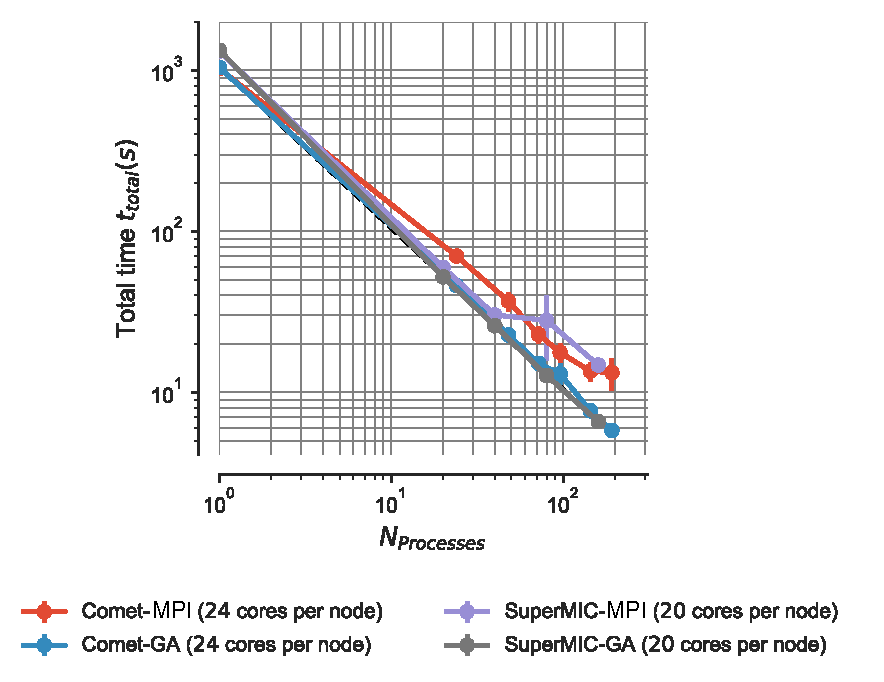
\includegraphics[width=\linewidth]{figures/Comparison_t-tot-clusters_Splitting_edited.pdf}
    \caption{Scaling total}
    \label{fig:MPIscaling-clusters-splitting}
  \end{subfigure}
  \hfill
  \begin{subfigure}{.49\textwidth}
    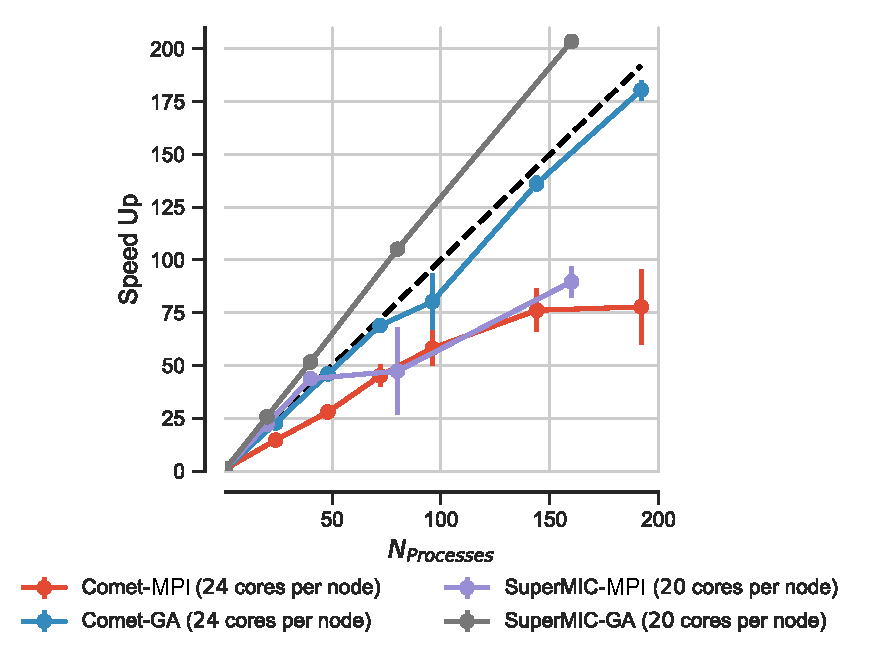
\includegraphics[width=\linewidth]{figures/Comparison_speed-up-clusters_Splitting_edited.pdf}
    \caption{Speed-up}
    \label{fig:MPIspeedup-clusters-splitting}
  \end{subfigure}
  \bigskip

  \begin{subfigure}{0.7\textwidth}
    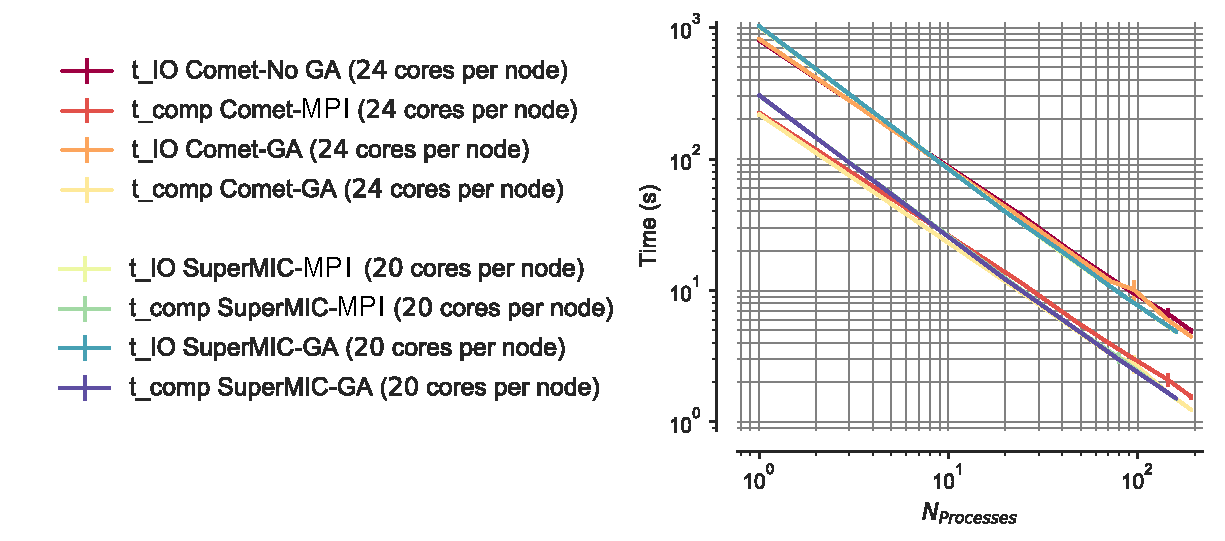
\includegraphics[width=\linewidth]{figures/Clusters_IO_compute_scaling_splitting_edited.pdf}
    \captionsetup{format=hang}
    \caption{Scaling of \tcomp and \tIO.}
    \label{fig:compute-IO-scaling-clusters-splitting}
  \end{subfigure}
  \caption{Comparison of the performance of the RMSD task ($\RcompIO \approx 0.3$) when the trajectories are split (subfiling) across different clusters (\emph{SDSC Comet}, \emph{LSU SuperMIC}.
    Results were communicated back to rank 0 either with MPI collective communications (label ``MPI'') or using \emph{Global Arrays} (label ``GA'').
    Five repeats were performed to collect statistics.
    The error bars show the standard deviation with respect to the mean.}
\label{fig:MPI-splitting-clusters}
\end{figure} 

\subsection{MPI-based Parallel HDF5}

Figure \ref{fig:MPIwithIO-clusters} shows the scaling on \emph{SDSC Comet}, \emph{LSU SuperMIC}, and \emph{PSC Bridges} using MPI-based parallel HDF5.  
Performance on \emph{SDSC Comet} and \emph{LSU SuperMIC} was very good with near ideal linear strong scaling.
The performance on \emph{PSC Bridges} was sensitive to how many cores per node were used.
Using all 28 cores in a node resulted in poor performance but decreasing the number of cores per node and equally distributing processes over nodes improved the scaling (Figure \ref{fig:MPIwithIO-clusters}), mainly by reducing variation in the I/O times.

The main difference between the runs on \emph{PSC Bridges} and \emph{SDSC Comet}/\emph{LSU SuperMIC} appeared to be the variance in \tIO (Figure \ref{fig:compute-IO-scaling-clusters}).
The I/O time distribution was fairly small and uniform across all ranks on \emph{SDSC Comet} and \emph{LSU SuperMIC} (Figures \ref{fig:hdf5-SuperMIC} and \ref{fig:MPIranks-hdf5}).
However, on \emph{PSC Bridges} the I/O time was on average about two and a half times larger and the I/O time distribution was also more variable across different ranks (Figure \ref{fig:hdf5-bridge}).  

\begin{figure}[!htb]
  \centering
  \begin{subfigure}{.49\textwidth}
    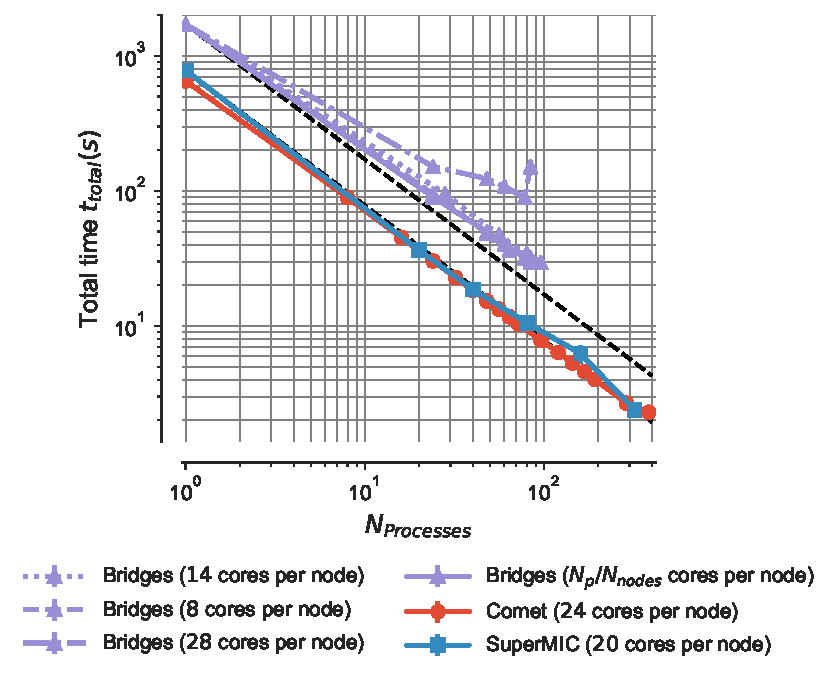
\includegraphics[width=\linewidth]{figures/Comparison_t-tot-clusters.pdf}
    \caption{Scaling total}
    \label{fig:MPIscaling-clusters}
  \end{subfigure}
  \hfill
  \begin{subfigure}{.49\textwidth}
    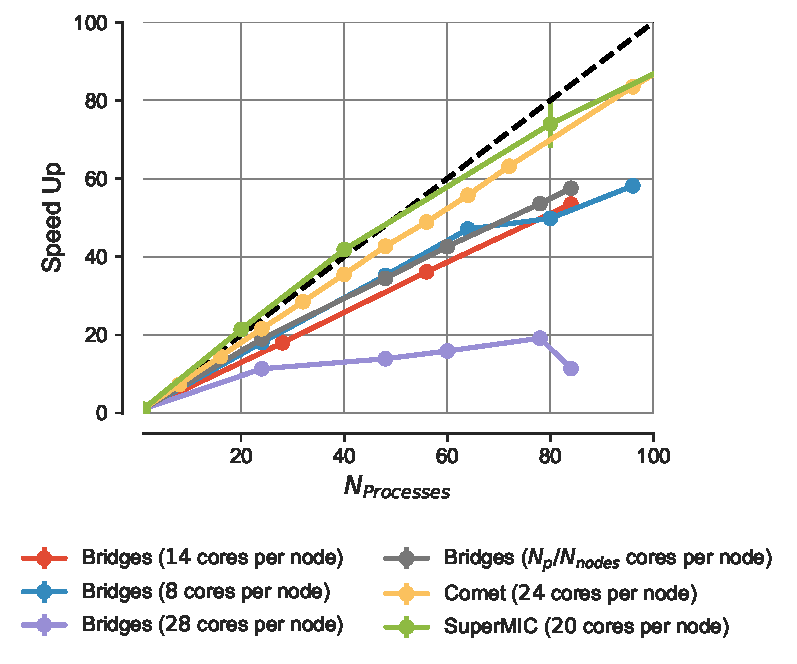
\includegraphics[width=\linewidth]{figures/Comparison_speed-up-clusters.pdf}
    \caption{Speed-up}
    \label{fig:MPIspeedup-clusters}
  \end{subfigure}
  \bigskip
  
  \begin{subfigure} {\textwidth}
    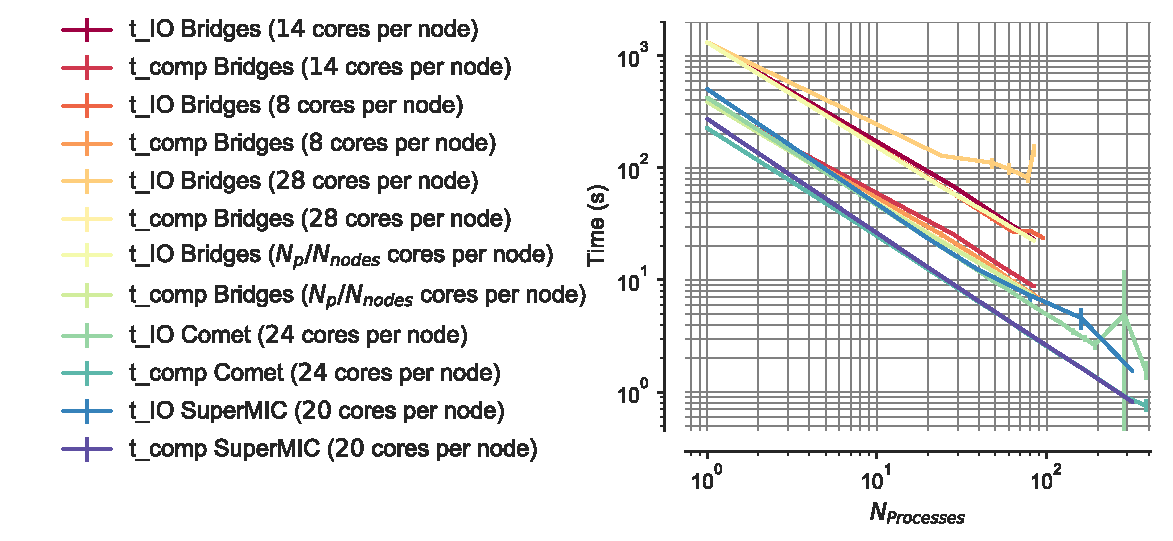
\includegraphics[width=\linewidth]{figures/Clusters_IO_compute_scaling_edited.pdf}
    \captionsetup{format=hang}
    \caption{Scaling of \tcomp and \tIO}
    \label{fig:compute-IO-scaling-clusters}
  \end{subfigure}
  \caption{Comparison of the performance of the RMSD task with MPI ($\RcompIO \approx 0.3$)  across different clusters (\emph{SDSC Comet}, \emph{PSC Bridges}, \emph{LSU SuperMIC}).
    Data were read from a shared HDF5 file instead of an XTC file, using MPI independent I/O.
    Results were communicated back to rank 0.
    $N_{\text{P}}/N_{\text{nodes}}$ indicates that number of processes used for the task were equally distributed over all compute nodes.
    Five repeats were performed to collect statistics.
    The error bars show standard deviation with respect to mean.
    In (b) only results up to 100 cores are shown to simplify the comparison; see Fig.~\protect\ref{fig:MPIspeedup-hdf5} for \emph{SDSC Comet} and Fig.~\protect\ref{fig:comparison_efficiency_SuperMIC} for \emph{LSU SuperMic} data.
  }
\label{fig:MPIwithIO-clusters}
\end{figure} 

\begin{figure}[!htb]
  \centering
  \begin{subfigure}{.49\textwidth}
    \includegraphics[width=\linewidth]{figures/Bridge-MPI-IO-BarPlot-rank-comparison_78_5.pdf}
    \caption{\emph{PSC Bridges}}
    \label{fig:hdf5-bridge}
  \end{subfigure}
  \bigskip
  \begin{subfigure} {.49\textwidth}
    \includegraphics[width=\linewidth]{figures/SuperMIC-MPI-IO-BarPlot-rank-comparison_80_5.pdf}
    \caption{\emph{LSU SuperMIC}}
    \label{fig:hdf5-SuperMIC}
  \end{subfigure}
  \caption{Examples of timing per MPI rank for RMSD task with MPI-based parallel HDF5 ($\RcompIO \approx 0.3$) on (a) \emph{PSC Bridges} and (b) \emph{LSU SuperMIC}.
    Five repeats were performed to collect statistics and these were typical data from one run of the 5 repeats. Compute \tcomp, read I/O \tIO, communication \tcomm, ending the for loop $t_{\text{end\_loop}}$,  opening the trajectory $t_{\text{opening\_trajectory}}$, and overheads $t_{\text{overhead1}}$, $t_{\text{overhead2}}$ per MPI rank; see Table \ref{tab:notation} for definitions.}
  \label{fig:MPIwithIO-clusters-rank}
\end{figure} 

\subsection{Comparison of Compute and I/O Scaling Across Different Clusters}
A full comparison of compute and I/O scaling across different clusters for different test cases and algorithms is shown in Table \ref{tab:comp-IO-scaling}. 
For MPI-based parallel HDF5, both the compute and I/O time on \emph{Bridges} were consistenly larger than their corresponding values on \emph{SDSC Comet} and \emph{LSU SuperMIC}.
For example, with one core the corresponding compute and I/O time were $\tcomp = 387~\text{s}$, $\tIO = 1318~\text{s}$ versus $225~\text{s}$, $423~\text{s}$ on \emph{SDSC Comet} and $273~\text{s}$, $503~\text{s}$ on \emph{LSU SuperMIC}.
This performance difference became larger with increasing core numbers.
When the trajectories were split and Global Arrays was used for communication both \emph{SDSC Comet} and \emph{LSU SuperMIC} showed similar performance.

Overall, the results from \emph{SDSC Comet} and \emph{LSU SuperMIC} are consistent with each other.
Performance on \emph{PSC Bridges} seemed sensitive to the exact allocation of cores on each node but nevertheless the approaches that decreased the occurence of stragglers on \emph{SDSC Comet} and \emph{LSU SuperMIC} also improved performace on \emph{PSC Bridges}.
Thus, the findings described in the previous sections are valid for a range of different HPC clusters with Lustre file systems.

\begin{sidewaystable}[hp]
\centering
\begin{adjustbox}{max width=\textwidth}
\begin{tabular}{c c c c c c c c c c c c}
  \toprule
 \multicolumn{10}{r}{\bfseries $N_{Processes}$} \\
\cmidrule(r){5-12}
           \bfseries\thead{Cluster} & \bfseries\thead{Gather} & \bfseries\thead{File Access} & \bfseries\thead{Time} & \bfseries\thead{Serial} & \begin{tabular}{c} \bfseries\thead{Comet:} 24 \\ \bfseries\thead{Bridges:} 24 \\ \bfseries\thead{SuperMIC:} 20 \end{tabular}  & \begin{tabular}{c} \bfseries\thead{Comet:} 48 \\ \bfseries\thead{Bridges:} 48 \\ \bfseries\thead{SuperMIC:} 40 \end{tabular} & \begin{tabular}{c} \bfseries\thead{Comet:} 72 \\ \bfseries\thead{Bridges:} 60 \\ \bfseries\thead{SuperMIC:} 80 \end{tabular} & \begin{tabular}{c} \bfseries\thead{Comet:} 96 \\ \bfseries\thead{Bridges:} 78 \end{tabular} & \begin{tabular}{c} \bfseries\thead{Comet:} 144 \\ \bfseries\thead{Bridges:} 84 \\ \bfseries\thead{SuperMIC:} 160\end{tabular} & \bfseries\thead{Comet: 192} & \begin{tabular}{c} \bfseries\thead{Comet:} 384 \\  \bfseries\thead{SuperMIC:} 320\end{tabular}\\
  \midrule
    Comet & MPI & Single & \begin{tabular}{c} \tIO \\ \tcomp  \end{tabular} & \begin{tabular}{c} $791 \pm 5.22$ \\ $225 \pm 5.4$ \end{tabular} & \begin{tabular}{c} $49 \pm 3.45$ \\ $11 \pm 0.75$ \end{tabular} & \begin{tabular}{c} $29 \pm 1.3$ \\ $6 \pm 0.35$ \end{tabular} & \begin{tabular}{c} $26 \pm 9.19$ \\ $4 \pm 0.48$ \end{tabular} & -- & -- & -- & --\\  
  \midrule
    Bridges & MPI & Single & \begin{tabular}{c} \tIO \\ \tcomp  \end{tabular} & \begin{tabular}{c} $770 \pm 10.8$ \\ $221 \pm 3.9$ \end{tabular} &  \begin{tabular}{c} $38 \pm 0.84$ \\ $11 \pm 0.43$ \end{tabular} & \begin{tabular}{c} $33 \pm 19.4$ \\ $6 \pm 0.32$ \end{tabular} & \begin{tabular}{c} $15 \pm 1.6$ \\ $4 \pm 0.18$ \end{tabular} & -- & -- & -- & --\\  
  \midrule
    SuperMIC & MPI & Single & \begin{tabular}{c} \tIO \\ \tcomp  \end{tabular} & \begin{tabular}{c} $1014.51 \pm 2.94$ \\ $303.85 \pm2.3$ \end{tabular} & \begin{tabular}{c} $48.08 \pm 0.35$ \\ $14.56 \pm 0.14$ \end{tabular} & \begin{tabular}{c} $24.5 \pm 0.79$ \\ $7.4 \pm 0.25$ \end{tabular} & \begin{tabular}{c} $12 \pm 0.31$ \\ $3.7 \pm 0.12$ \end{tabular} & -- & \begin{tabular}{c} $6.24 \pm 0.38$ \\ $1.8 \pm 0.04$ \end{tabular} & -- & --\\  
  \midrule
    Comet & GA & Single & \begin{tabular}{c} \tIO \\ \tcomp \end{tabular} & \begin{tabular}{c} $820 \pm 18.49$ \\ $219 \pm 9.8$ \end{tabular} & \begin{tabular}{c} $41 \pm 8.99$ \\ $10 \pm 0.3$ \end{tabular} & \begin{tabular}{c} $23 \pm 4.14$ \\ $5 \pm 0.48$ \end{tabular} & \begin{tabular}{c} $15 \pm 2.06$ \\ $3 \pm 0.54$ \end{tabular} & -- & -- & -- & --\\
  \midrule
    Comet & MPI & Splitting & \begin{tabular}{c} \tIO \\ \tcomp \end{tabular} & \begin{tabular}{c} $799 \pm 5.22$ \\ $225 \pm 5.4$ \end{tabular} & \begin{tabular}{c} $37 \pm 1.22$ \\ $11 \pm 0.31$ \end{tabular} & \begin{tabular}{c} $18 \pm 0.18$ \\ $5 \pm 0.07$ \end{tabular} & \begin{tabular}{c} $12 \pm 0.14$ \\ $3 \pm 0.04$ \end{tabular} & \begin{tabular}{c} $9 \pm 0.3$ \\ $3 \pm 0.11$ \end{tabular} & \begin{tabular}{c} $6  \pm 0.66$ \\ $2 \pm 0.23$ \end{tabular} & \begin{tabular}{c} $4 \pm 0.23$ \\ $1 \pm 0.07$ \end{tabular} & --\\
  \midrule
    SuperMIC &  MPI & Splitting & \begin{tabular}{c} \tIO \\ \tcomp \end{tabular} & \begin{tabular}{c} $1013.75 \pm 2.8$ \\ $304.26 \pm 2.55$ \end{tabular} & \begin{tabular}{c} $39.99 \pm 0.36$ \\ $12.41 \pm 0.22$ \end{tabular} & \begin{tabular}{c} $19.18 \pm 0.25$ \\ $5.99\pm 0.09$ \end{tabular} & \begin{tabular}{c} $9.61 \pm 0.28$ \\ $3.08 \pm 0.13$ \end{tabular} & -- & \begin{tabular}{c} $4.83 \pm 0.06$ \\ $1.5 \pm 0.01$ \end{tabular} & --& --\\ 
  \midrule 
    Comet &  GA & Splitting & \begin{tabular}{c} \tIO \\ \tcomp \end{tabular} & \begin{tabular}{c} $820 \pm 18.5$ \\ $219 \pm 9.5$ \end{tabular} & \begin{tabular}{c} $36 \pm 0.78$ \\ $9 \pm 0.22$ \end{tabular} & \begin{tabular}{c} $17 \pm 0.3$ \\ $4 \pm 0.07$ \end{tabular} & \begin{tabular}{c} $11 \pm 0.23$ \\ $3 \pm 0.04$ \end{tabular} & \begin{tabular}{c} $10 \pm 1.7$ \\ $2 \pm 0.4$ \end{tabular} & \begin{tabular}{c} $5 \pm 0.14$ \\ $1 \pm 0.05$ \end{tabular} & \begin{tabular}{c} $4 \pm 0.07$ \\ $1 \pm 0.02$ \end{tabular} & --\\
  \midrule
    SuperMIC & GA & Splitting & \begin{tabular}{c} \tIO \\ \tcomp \end{tabular} & \begin{tabular}{c} $1027.62 \pm 10.32$ \\ $305.78 \pm 3.47$ \end{tabular} & \begin{tabular}{c} $39.62 \pm 0.2$ \\ $12.16 \pm 0.1$ \end{tabular} & \begin{tabular}{c} $19.66 \pm 0.1$ \\ $6.01\pm 0.007$ \end{tabular} & \begin{tabular}{c} $9.57 \pm 0.1$ \\ $2.97 \pm 0.1$ \end{tabular} & -- & \begin{tabular}{c} $4.86 \pm 0.05$ \\ $1.51 \pm 0.03$ \end{tabular} & --& --\\     
  \midrule
    Comet & MPI & PHDF5 & \begin{tabular}{c} \tIO \\ \tcomp \end{tabular} & \begin{tabular}{c} $423 \pm 5.88$ \\ $225 \pm 6.55$ \end{tabular} & \begin{tabular}{c} $19 \pm 0.3$ \\ $10 \pm 0.12$ \end{tabular} & \begin{tabular}{c} $9 \pm 0.13$ \\ $5 \pm 0.1$ \end{tabular} & \begin{tabular}{c} $6 \pm 0.06$ \\ $3 \pm 0.04$ \end{tabular} & \begin{tabular}{c} $5 \pm 0.12$ \\ $2 \pm 0.05$ \end{tabular} & \begin{tabular}{c} $3 \pm 0.2$ \\ $1 \pm 0.04$ \end{tabular} & \begin{tabular}{c} $3 \pm 0.25$\\ $1 \pm 0.03$ \end{tabular} & \begin{tabular}{c} $1.57 \pm 0.29$\\ $0.76 \pm 0.09$ \end{tabular}\\
  \midrule 
    Bridges & MPI & PHDF5 & \begin{tabular}{c} \tIO \\ \tcomp \end{tabular} & \begin{tabular}{c} $1318.87 \pm 10.42$ \\ $387.8 \pm 5.51$ \end{tabular} & \begin{tabular}{c} $67.93 \pm 0.52$ \\ $21.97 \pm 0.38$ \end{tabular} & \begin{tabular}{c} $37.37 \pm 0.2$ \\ $12.12 \pm 0.34$ \end{tabular} & \begin{tabular}{c} $30.35 \pm 0.15$ \\ $9.79 \pm 0.24$ \end{tabular} & \begin{tabular}{c} $24.16 \pm 0.89$ \\ $7.72 \pm 0.03$ \end{tabular} & \begin{tabular}{c} $22.5 \pm 0.17$ \\ $7.18 \pm 0.08$ \end{tabular} & -- & --\\ 
  \midrule
    SuperMIC & MPI & PHDF5 & \begin{tabular}{c} \tIO \\ \tcomp \end{tabular} & \begin{tabular}{c} $503.69 \pm 2.57$ \\ $273.54 \pm 4.7$ \end{tabular} & \begin{tabular}{c} $12.96 \pm 0.06$ \\ $23.44 \pm 0.29$ \end{tabular} & \begin{tabular}{c} $6.46 \pm 0.02$ \\ $12.22 \pm 0.43$ \end{tabular} & \begin{tabular}{c} $3.2 \pm 0.01$ \\ $7.3 \pm 0.85$ \end{tabular} & -- & \begin{tabular}{c} $1.64 \pm 0.01$ \\ $4.59 \pm 0.96$ \end{tabular} & --& \begin{tabular}{c} $0.82 \pm 0.004$ \\ $1.55 \pm 0.009$ \end{tabular} \\
  \bottomrule
\end{tabular}
\end{adjustbox}
\caption
{Comparison of the compute and I/O scaling for different test cases and number of processes.
  Five repeats were performed to collect statistics.
  The mean value and the standard deviation with respect to mean are reported for each case.}
\label{tab:comp-IO-scaling}
\end{sidewaystable}



\section{Guidelines for Improving Parallel Trajectory Analysis Performance}
% -*- mode: latex; mode: visual-line; fill-column: 9999; coding: utf-8 -*-

\section{Guidelines for Improving Parallel Trajectory Analysis Performance}
\label{sec:guidelines}

Although the performance measurements were performed with \package{MDAnalysis} and therefore capture some details of this library such as the sepecific timings for file reading, we believe that the broad picture is fairly general and applies to any Python-based approach that uses MPI for parallelizing trajectory access with a split-apply-combine approach.
Based on the lessons that we learned, we suggest the following guidelines to improve strong scaling performance:
\begin{description}
\item[\textbf{Heuristic 1}] Calculate compute to I/O ratio ($\RcompIO$, Eq.~\ref{eq:Compute-IO}) and compute to communication ratio ($\Rcompcomm$, Eq.~\ref{eq:Compute-comm}).
  $\RcompIO$ determines whether the task is compute bound ($\RcompIO \gg 1$) or IO bound ($\RcompIO \ll 1$).
  $\Rcompcomm$ determines whether the task is communication bound ($\frac{\overline{\tcomp}}{\overline{\tcomm}} \ll 1$) or compute bound ($\RcompIO \gg 1$).

  As discussed in Section \ref{sec:bound}, for I/O bound problems the interference between MPI communication and I/O traffic can be problematic \cite{VMD2013, Brown:2018ab} and the performance of the task will be affected by the straggler tasks that delay job completion time.
  
\item[\textbf{Heuristic 2}] For $\RcompIO \ge 1$, single-shared-file I/O can be used and will not decrease performance. One may consider the following cases: 
  \begin{description}
  \item[\textbf{Heuristic 2.1}] If $\Rcompcomm \gg 1$, the task is compute bound and will scale well as shown in Figure \ref{fig:tcomp_tIO_effect}. 
  \item[\textbf{Heuristic 2.2}] If $\Rcompcomm \ll 1$, one might consider using \package{Global Arrays} to improve scaling by utilizing efficient distribution of data via the shared arrays (section \ref{Global-Array}).
  \end{description}
\item[\textbf{Heuristic 3}] For $\RcompIO \le 1$ the task is I/O bound and single-shared-file I/O should be avoided to remove unnecessary metadata operations.
  One might want to consider the following steps:  
  \begin{description}
    \item[\textbf{Heuristic 3.1}] If there is access to HDF5 format, use MPI-based Parallel HDF5 (Section \ref{HDF5}). 
    \item[\textbf{Heuristic 3.2}] If the trajectory file is not in HDF5 format then one can consider subfiling and split the single trajectory file into as many trajectory segments as the number of processes.
      Splitting the trajectories can be easily performed in parallel and trajectory conversion may be integrated into the beginning of standard workflows for MD simulations.
      Alternatively, trajectories may be kept in smaller chunks if they are already produced in batches; for instance, when running simulations with \package{Gromacs} \cite{Abraham:2015aa}, the \texttt{gmx mdrun -noappend} option produces individual trajectory segments instead of extending an existing trajectory file.
    \item[\textbf{Heuristic 3.3}] In case of $\Rcompcomm \ll 1$, use of \package{Global Arrays} may be considered to potentially improve scaling (Section \ref{splitting-traj}).
  \end{description}
\end{description}


\section{Conclusions}
% -*- mode: latex; mode: visual-line; fill-column: 9999; coding: utf-8 -*-

\section{Conclusions}
\label{sec:conclusions}

We analyzed the strong scaling performance of a typical task when analysing MD trajectories, the calculation of the time series of the RMSD of a protein, with the widely used Python-based \package{MDAnalysis} library.
The task was parallelized with MPI following the \emph{split-apply-combine} approach by having each MPI process analyze a contiguous segment of the trajectory.
This approach did not scale beyond a single node because straggler MPI processes exhibited large upward variations in runtime.
Stragglers were primarily caused by either increased MPI communication costs or increased time to open the single shared trajectory file whereas both the computation and the ingestion of data exhibited close to ideal strong scaling behavior.
Stragglers were less prevalent for compute-bound workloads (i.e., $\RcompIO \gg 1$), suggesting that file read I/O was responsible for poor MPI communication.
In particular, artifically removing all I/O substantially improved performance of the communication step and thus brought overall performance close to ideal (i.e., linear increase in speed-up with processor count with slope one).
By performing benchmarks on three different XSEDE supercomputers we showed that our results were independent from the specifics of the hardware and local environment.
Our results hint at the possibility that stragglers might be due to the competition between MPI messages and the Lustre file system on the shared InfiniBand interconnect, which would be consistent with other similar observations \cite{VMD2013} and theoretical predictions by \citet{Brown:2018ab}.
One possible interpretation of our results is that for a sufficiently large per-frame compute workload, read I/O interferes much less with communication than for an I/O bound task that almost continuously accesses the file system.
This intepretation suggested that we needed to improve read I/O to reduce interference.

We investigated subfiling (splitting of the trajectories into separate files, one for each MPI rank) and MPI-based parallel I/O.
Subfiling improved scaling, especially when combined with the \package{Global Arrays} toolkit.
Somewhat surprisingly\mknote{I really disagree we this sentence. I do not understand why the results of the GA is surprising for every one. I have tried to explain why GA lead to better perforance. What is not clear to you?}, \package{Global Arrays} reduced the communication cost compared to MPI collective communications even though it only acts as programming layer to access data across multiple nodes in a convenient array form and also uses MPI for its inter-node data exchange.
Subfiling with \package{Global Arrays} achieved nearly ideal scaling up to 192 cores (8 nodes on \emph{SDSC Comet}).
When we used MPI-based parallel I/O through HDF5 together with MPI for communications we achieved nearly ideal performance up to 384 cores (16 nodes on \emph{SDSC Comet}) and speed-ups of two orders of magnitude compared to the serial execution.
The latter approach appears to be a promising way forward as it directly builds on very widely used technology (MPI-IO and HDF5) and echoes the experience of the wider HPC community that parallel file I/O is necessary for efficient data handling.

The biomolecular simulation community suffers from a large number of trajectory file formats with very few being based on HDF5, with the exception of the H5MD format \cite{Buyl:2014aa} and the MDTraj HDF5 format \cite{McGibbon:2015aa}.
Our work suggests that HDF5-based formats should be seriously considered as the default for MD simulations if users want to make efficient use of their HPC systems for analysis. 
Alternatively, enabling MPI-IO for trajectory readers in libraries such as \package{MDAnalysis} might also provide a path forward to better read performance.

We summarized our findings in a number of guidelines for improving the scaling of parallel analysis of MD trajectory data.
We showed that it is feasible to run an I/O bound analysis task on HPC resources with a Lustre parallel filesystem and achieve good scaling behavior up to 384 CPU cores with an almost 300-fold speed-up compared to serial execution.
Although we focused on the \package{MDAnalysis} library, similar strategies are likely to be more generally applicable and useful to the wider biomolecular simulation community.





\subsection*{Acknowledgements}
\label{acknowledgements}


We are grateful to Sarp Oral for insightful comments on this manuscript.
This work was supported by the National Science Foundation under grant numbers ACI-1443054 and ACI-1440677.
This work used the Extreme Science and Engineering Discovery Environment (XSEDE), which is supported by National Science Foundation grant number ACI-1548562.
\emph{SDSC Comet} at the San Diego Supercomputer Center, \emph{LSU SuperMic} at Louisiana State University, and \emph{PSC Bridges} at the Pittsburgh Supercomputing Center were used under allocations TG-MCB090174 and TG-MCB130177.

\section*{References}

\bibliography{main}

\clearpage

\appendix
\section{Additional Data}
\label{sec:supplement}

Figure \ref{fig:MPIwithIO-Bridges} shows performance of the RMSD task on \emph{PSC Bridges}. 

\begin{figure}[!htb]
  \centering
  \begin{subfigure}{.4\textwidth}
    \includegraphics[width=\linewidth]{figures/main-RMSD-t_total-Bridges.pdf}
    \caption{Scaling total (five repeats)}
    \label{fig:MPIscaling-Bridges}
  \end{subfigure}
  \hfill
  \begin{subfigure}{.4\textwidth}
    \includegraphics[width=\linewidth]{figures/main-RMSD-speed_up-Bridges.pdf}
    \caption{Speed-up (five repeats)}
    \label{fig:MPIspeedup-Bridges}
  \end{subfigure}
  \bigskip

  \begin{subfigure}{.4\textwidth}
    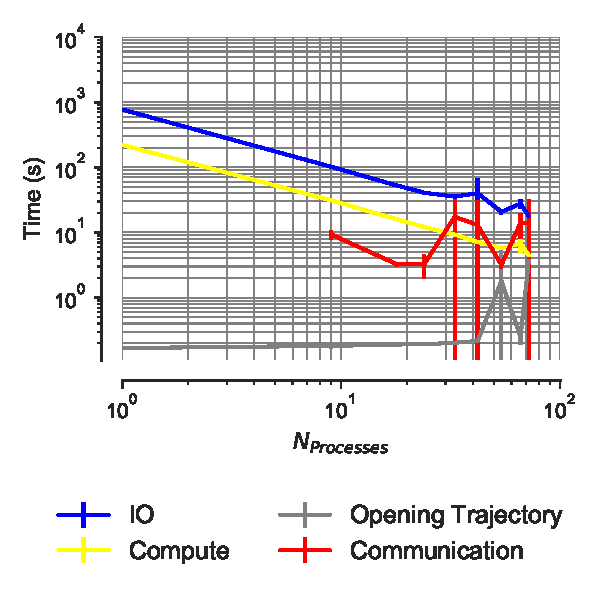
\includegraphics[width=\linewidth]{figures/main-RMSD-time_comp_IO_comparison-Bridges.pdf}
    \captionsetup{format=hang}
    \caption{Scaling for different components (five repeats)}
    \label{fig:ScalingComputeIO-Bridges}
  \end{subfigure}
  \hfill
  \begin{subfigure} {.5\textwidth}
    \includegraphics[width=\linewidth]{figures/main-RMSD-BarPlot-rank-comparison_72_4-Bridges.pdf}
    \captionsetup{format=hang}
    \caption{Time comparison on different parts of the calculations per MPI rank (example)}
    \label{fig:MPIranks-Bridges}
  \end{subfigure}
  \caption{\emph{PSC Bridges}: Performance of the RMSD task with MPI.
    Results are communicated back to rank 0.
    Five independent repeats were performed to collect statistics.
    (a-c) The error bars show standard deviation with respect to mean. (d) Compute \tcomp, IO \tIO, communication \tcomm, ending the for loop $t_{\text{end\_loop}}$, opening the trajectory $t_{\text{opening\_trajectory}}$, and overheads $t_{\text{overhead1}}$, $t_{\text{overhead2}}$ per MPI rank; see Table \ref{tab:notation} for definitions.
    These are data from one run of the five repeats.
    MPI ranks 0 and 70 are stragglers.
    Note: In serial, there is no communication and hence no data point is shown for $N=1$.}
\label{fig:MPIwithIO-Bridges}
\end{figure} 



Figure \ref{fig:MPIwithIO-SuperMIC} shows performance of the RMSD task on \emph{LSU SuperMIC}. 

\begin{figure}[!htb]
  \centering
  \begin{subfigure}{.4\textwidth}
    \includegraphics[width=\linewidth]{figures/main-RMSD-t_total-SuperMIC.pdf}
    \caption{Scaling total (five repeats)}
    \label{fig:MPIscaling-SuperMIC}
  \end{subfigure}
  \hfill
  \begin{subfigure}{.4\textwidth}
    \includegraphics[width=\linewidth]{figures/main-RMSD-speed_up-SuperMIC.pdf}
    \caption{Speed-up (five repeats)}
    \label{fig:MPIspeedup-SuperMIC}
  \end{subfigure}
  \bigskip

  \begin{subfigure}{.4\textwidth}
    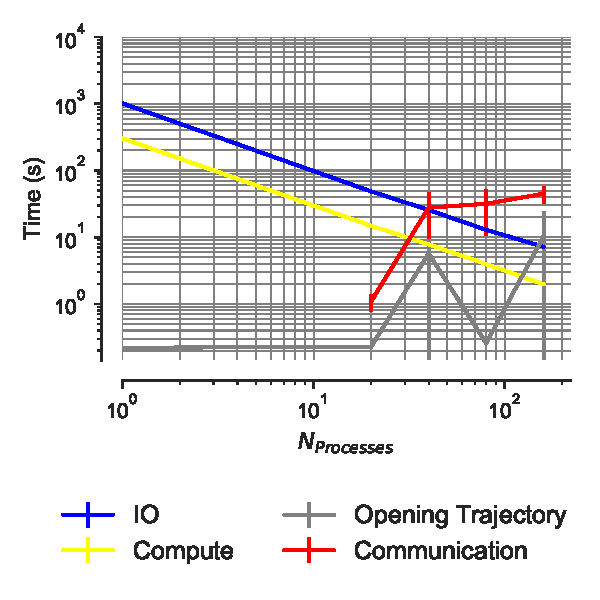
\includegraphics[width=\linewidth]{figures/main-RMSD-time_comp_IO_comparison-SuperMIC.pdf}
    \captionsetup{format=hang}
    \caption{Scaling for different components (five repeats)}
    \label{fig:ScalingComputeIO-SuperMIC}
  \end{subfigure}
  \hfill
  \begin{subfigure} {.5\textwidth}
    \includegraphics[width=\linewidth]{figures/main-RMSD-BarPlot-rank-comparison_80_5-SuperMIC.pdf}
    \captionsetup{format=hang}
    \caption{Time comparison on different parts of the calculations per MPI rank (example)}
    \label{fig:MPIranks-SuperMIC}
  \end{subfigure}
  \caption{\emph{LSU SuperMIC}: Performance of the RMSD task with MPI.
    Results are communicated back to rank 0.
    Five independent repeats were performed to collect statistics.
    (a-c) The error bars show standard deviation with respect to mean.
    (d) Compute \tcomp, IO \tIO, communication \tcomm, ending the for loop $t_{\text{end\_loop}}$,  opening the trajectory $t_{\text{opening\_trajectory}}$, and overheads $t_{\text{overhead1}}$, $t_{\text{overhead2}}$ per MPI rank; see Table \ref{tab:notation} for definitions.
    These are data from one run of the five repeats.
    MPI ranks 0 and 70 are stragglers.
    Note: In serial, there is no communication and hence the data points for $N=1$ are not shown.}
  \label{fig:MPIwithIO-SuperMIC}
\end{figure} 


Figure \ref{fig:comparison_efficiency_clusters} shows comparison of the parallel efficiency of the RMSD task between different test cases on \emph{SDSC Comet}, \emph{PSC Bridges}, and \emph{LSU SuperMIC}.  

\begin{figure}[!htb]
  \centering
  \begin{subfigure}{.3\textwidth}
    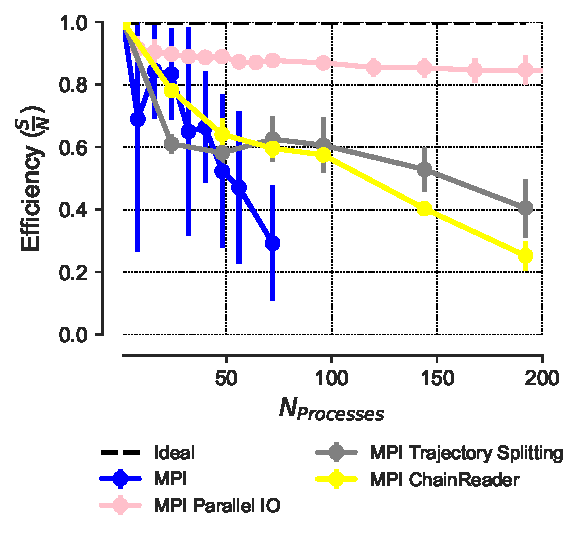
\includegraphics[width=\linewidth]{figures/Comparison_Efficiency_all_Comet.pdf}
    \caption{\emph{SDSC Comet}}
    \label{fig:comparison_efficiency}
  \end{subfigure}
  \hfill
  \begin{subfigure}{.35\textwidth}
    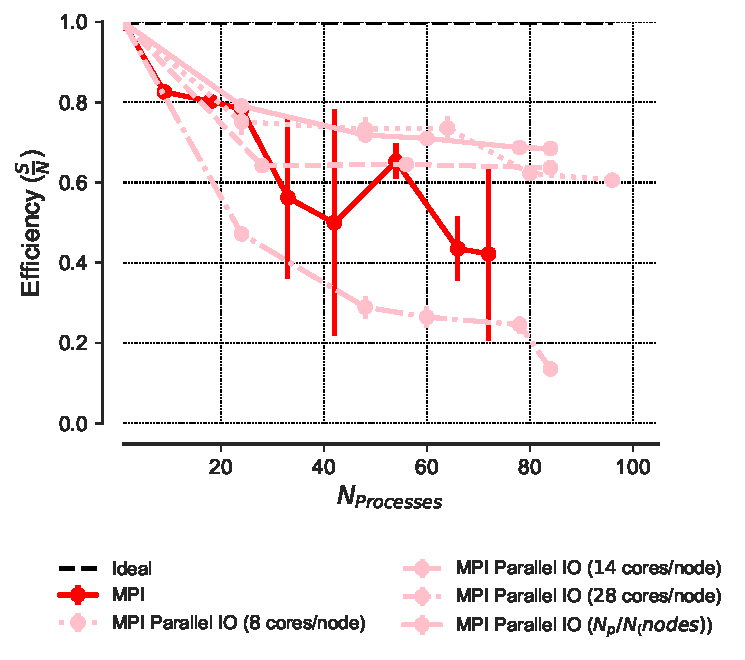
\includegraphics[width=\linewidth]{figures/Comparison_Efficiency_all_Bridges.pdf}
    \caption{\emph{PSC Bridges}}
    \label{fig:comparison_efficiency_Bridges}
  \end{subfigure}
  \hfill
  \begin{subfigure}{.3\textwidth}
    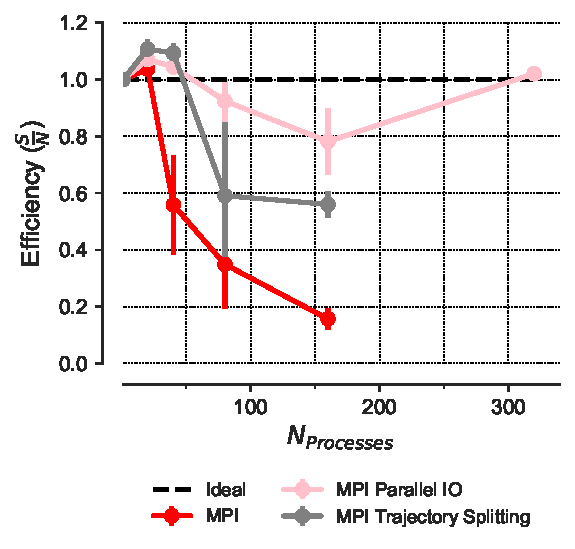
\includegraphics[width=\linewidth]{figures/Comparison_Efficiency_all_SuperMIC.pdf}
    \caption{\emph{LSU SuperMIC}}
    \label{fig:comparison_efficiency_SuperMIC}
  \end{subfigure}
  \caption{Comparison of the parallel efficiency between different test cases on (a) \emph{SDSC Comet}, (b) \emph{PSC Bridges}, and (c) \emph{LSU SuperMIC}.
    Five repeats were performed to collect statistics and error bars show standard deviation with respect to mean.}
  \label{fig:comparison_efficiency_clusters}
\end{figure} 

Figure \ref{fig:MPIwithIO-split-SuperMIC} shows how RMSD task scales with the increase in the number of cores when the trajectories are split using \emph{Global Arrays} for communication compared to using MPI for communications on \emph{LSU SuperMIC}.  
 
\begin{figure}[!htb]
  \centering
  \begin{subfigure}{.3\textwidth}
    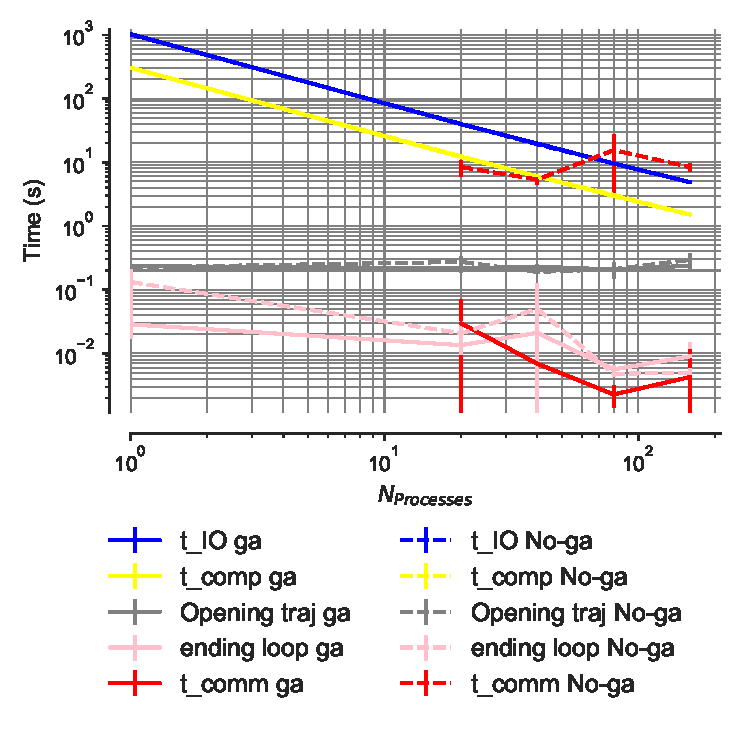
\includegraphics[width=\linewidth]{figures/Comparison_IO_compute_scaling_traj_splitting-SuperMIC.pdf}
    \captionsetup{format=hang}
    \caption{Scaling for different components}
    \label{fig:MPIscaling-SuperMIC}
  \end{subfigure}
  \hfill
  \begin{subfigure}{.3\textwidth}
    \includegraphics[width=\linewidth]{figures/Comparison_tot_time_traj_splitting-SuperMIC.pdf}
    \caption{Scaling total}
    \label{fig:MPItottime-SuperMIC}
  \end{subfigure}
  \hfill
  \begin{subfigure}{.3\textwidth}
    \includegraphics[width=\linewidth]{figures/Comparison_Speed_UP_traj_splitting-SuperMIC.pdf}
    \caption{Speed-up}
    \label{fig:MPIspeedup-SuperMIC}
  \end{subfigure}

  \caption{\emph{LSU SuperMIC}: Comparison on the performance of the RMSD task with MPI with subfiling and using either \emph{Global Arrays} for communication (``ga'') or using MPI as before (``No-ga'').
    For \emph{Global Arrays}, all ranks update the global array (\texttt{ga\_put()}) and rank 0 accesses the whole RMSD array through the global memory address (\texttt{ga\_get()}).
    Five repeats were performed to collect statistics.
    (a) Compute and I/O scaling versus number of processes.
    (b) Total time scaling versus number of processes.
    (c) Speed-up.
    (a-c) The error bars show standard deviation with respect to mean.}
  \label{fig:MPIwithIO-split-SuperMIC}
\end{figure}



\section{Effect of \Rcompcomm on Performance}
% -*- mode: latex; mode: visual-line; fill-column: 9999; coding: utf-8 -*-

\section{Effect of \Rcompcomm on Performance}
\label{sec:tcomm}

In Section \ref{sec:I/O}, we improved scaling limitations due to read I/O by splitting the trajectory, but scaling remained far from ideal when MPI communication was used; somewhat surprisingly, using \emph{Global Arrays} lead to better scaling (see Section \ref{Global-Array}) because the effective communication cost was reduced \mknote{I really disagree we this sentence. I do not understand why the results of the GA is surprising for every one. I have tried to explain why GA lead to better perforance. What is not clear to you?}.
Although we were not able to identify the reason for the better performance of \emph{Global Arrays} (it still uses MPI as a communicator), the results motivated an analysis in terms of the communication costs.
In addition to the compute to I/O ratio \RcompIO discussed in Section \ref{sec:bound} we defined another performance parameter called the compute to communication ratio $\Rcompcomm$ (Eq.~\ref{eq:Compute-comm}).

We analyzed the data for variable workloads (see Section \ref{sec:bound}) in terms of the $\Rcompcomm$ ratio.
The performance clearly depended on the $\Rcompcomm$ ratio (Figure \ref{fig:tcom_tcomm_effect}).
Performance improved with increasing $\Rcompcomm$ ratios (Figure \ref{fig:tcomp_tcomm_ratio} and \ref{fig:S1_tcomp_tcomm_effect}) even if the communication time was larger (Figure \ref{fig:Comm_time_tcomp_tcomm_effect}).
Although we still observed stragglers due to communication at larger $\Rcompcomm$ ratios ($70\times$ RMSD and $100\times$ RMSD), their effect on performance remained modest because the overall performance was dominated by the compute load. 
Evidently, as long as overall performance is dominated by a component such as compute that scales well, then performance problems with components such as communication will be masked and overall acceptable performance can still be achieved (Figures \ref{fig:S1_tcomp_tcomm_effect} and \ref{fig:tcomp_tcomm_ratio}).

Communication was usually not problematic within one node because of the shared memory environment.
For less than 24 processes, i.e., a single compute node on \emph{SDSC Comet}, the scaling was good and $\Rcompcomm \gg 1$ for all RMSD loads (Figures \ref{fig:S1_tcomp_tcomm_effect} and \ref{fig:tcomp_tcomm_ratio}).
However, beyond a single compute node ($>$ 24 cores), scaling appeared to improve with increasing $\Rcompcomm$ ratio while the communication overhead decreased in importance (Figures \ref{fig:S1_tcomp_tcomm_effect} and \ref{fig:tcomp_tcomm_ratio}).

\begin{figure}[!htb]
  \centering
  \begin{subfigure} {.33\textwidth}
    \includegraphics[width=\linewidth]{figures/Compute_to_IO_ratio_on_performance_2d_v17.pdf}
    \caption{Speed-Up $S(N)$}
    \label{fig:S1_tcomp_tcomm_effect}
  \end{subfigure}
  \hfill
  \begin{subfigure}{.3\textwidth}
    \includegraphics[width=\linewidth]{figures/Compute_to_comm_ratio_on_performance_v17.pdf}
    \captionsetup{format=hang}
    \caption{Compute to communication ratio \Rcompcomm}
    \label{fig:tcomp_tcomm_ratio}
  \end{subfigure}
  \hfill
  \begin{subfigure}{.33\textwidth}
    \includegraphics[width=\linewidth]{figures/comm_comparison_different_RMSD_overload.pdf}
    \caption{Communication time \tcomm}
    \label{fig:Comm_time_tcomp_tcomm_effect}
  \end{subfigure}
  \caption{Effect of the ratio of compute to communication time \Rcompcomm on scaling performance on \emph{SDSC Comet}.
    (a) Scaling for different computational workloads. (Same as Figure~\protect\ref{fig:S1_tcomp_tIO_effect}.)
    (b) Change in \Rcompcomm with the number of processes $N$ for different workloads. 
    (c) Comparison of communication time for different RMSD workloads.
    Five repeats were performed to collect statistics and error bars show standard deviation with respect to mean.}
  \label{fig:tcom_tcomm_effect}
\end{figure}

%%% Local Variables:
%%% mode: latex
%%% TeX-master: t
%%% End:


\section{Performance of the ChainReader for Split Trajectories}
% -*- mode: latex; mode: visual-line; fill-column: 9999; coding: utf-8 -*-

\section{Performance of the ChainReader for Split Trajectories}
\label{sec:chainreader}

In section \ref{sec:splitting-traj} we showed how subfiling (splitting the trajectories) would help to overcome I/O limitations and improve scaling. 
However, the number of trajectories may not necessarily be equal to the number of processes.
For example, trajectories from MD simulations on supercomputers are often kept in small segments in individual files that need to be concatenated later to form a trajectory that can be analyzed with common tools.
Such segments might be useful for subfiling but making sure that the number of processes is equal to the number of trajectory files will not always be feasible. 
\package{MDAnalysis} can transparently represent multiple trajectories as one virtual trajectory using the \emph{ChainReader}.
This feature is  convenient for serial analysis when trajectories are maintained as segments.
In the current implementation of ChainReader, each process opens all the trajectory segment files but I/O will only happen from a specific block of the trajectory specific to that process only.

We wanted to test if the ChainReader would benefit from the gains measured for the subfiling approach.
Specifically, we measured if the MPI-parallelized RMSD task (with $N_{\text{p}}$ ranks) would benefit if the trajectory was split into $N_{\text{seg}} = N_{\text{p}}$ trajectory segments, corresponding to an ideal scenario.
 
 \begin{figure}[!htb]
\centering
\begin{subfigure}{.3\textwidth}
  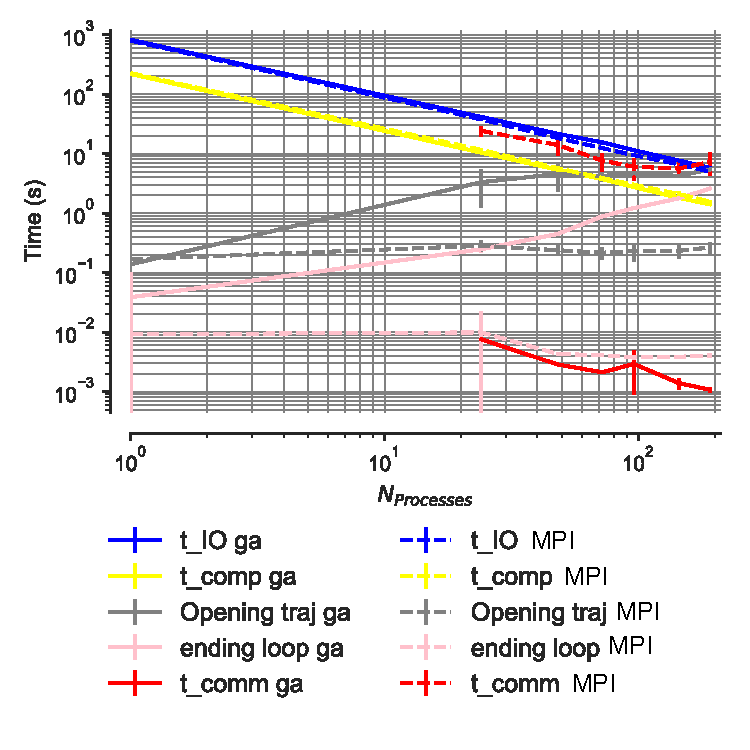
\includegraphics[width=\linewidth]{figures/Comparison_IO_compute_scaling_traj_splitting-chain-reader_edited.pdf}
  \captionsetup{format=hang}
  \caption{Scaling for different components}
  \label{fig:MPIscaling-chain-reader}
\end{subfigure}
\hfill
\begin{subfigure}{.3\textwidth}
  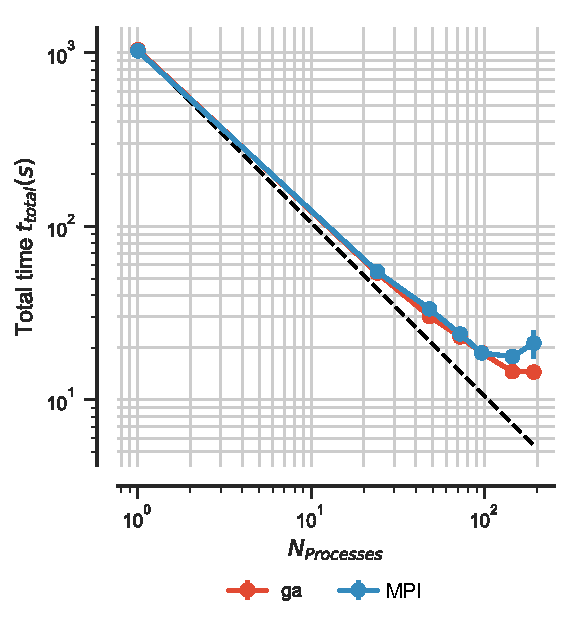
\includegraphics[width=\linewidth]{figures/Comparison_tot_time_traj_splitting-chain-reader_edited.pdf}
  \caption{Scaling total}
  \label{fig:MPItottime-chain-reader}
\end{subfigure}
\hfill
\begin{subfigure}{.3\textwidth}
  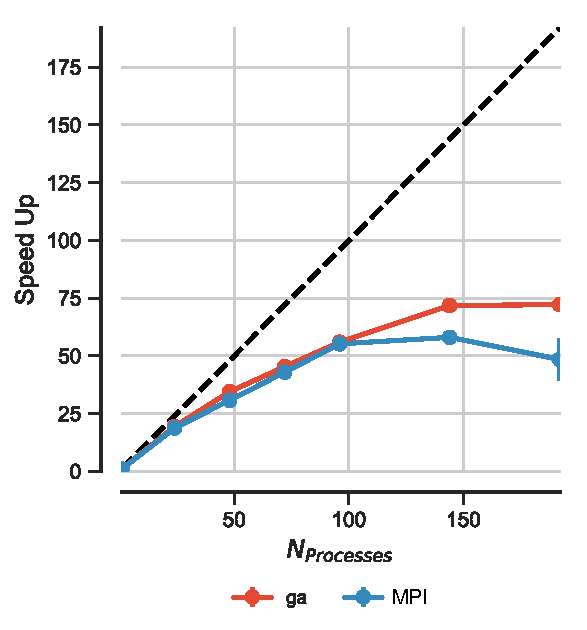
\includegraphics[width=\linewidth]{figures/Comparison_Speed_UP_traj_splitting-chain-reader_edited.pdf}
  \caption{Speed-up}
  \label{fig:MPIspeedup-chain-reader}
\end{subfigure}
\bigskip

\begin{subfigure}{.45\textwidth}
  \includegraphics[width=\linewidth]{figures/chain-reader-no-ga-BarPlot-rank-comparison_192_5.pdf}
  \captionsetup{format=hang}
   \caption{Time comparison of different parts of the calculations per MPI rank using ChainReader with MPI collective communications}
  \label{fig:MPIranks-split-chain-reader}
\end{subfigure}
\hfill
\begin{subfigure}{.45\textwidth}
  \includegraphics[width=\linewidth]{figures/chain-reader-ga-BarPlot-rank-comparison_192_3.pdf}
  \captionsetup{format=hang}
  \caption{Time comparison on different parts of the calculations per MPI rank using ChainReader using \package{Global Arrays}}
  \label{fig:MPIranks-split-ga-chain-reader}
\end{subfigure}

\caption{Comparison on the performance of the MDAnalysis ChainReader for the RMSD task on \emph{SDSC Comet} when the trajectories are split; for the communication step either collective MPI (``MPI'') or \package{Global Arrays} (``ga'') was used.
In case of \package{Global Arrays}, all ranks update the global array (\texttt{ga\_put()}) and rank 0 accesses the whole RMSD array through the global memory address (\texttt{ga\_get()}).
Five repeats were performed to collect statistics.
(a) Compute and I/O scaling versus number of processes.
(b) Total time scaling versus number of processes.
(c) Speed-up.
(a-c) The error bars show standard deviation with respect to the mean.
(d-e) Compute \tcomp, read I/O \tIO, communication \tcomm, access to the whole global array by rank 0 $t_{\text{Access\_Global\_Array}}$, ending the for loop $t_{\text{end\_loop}}$,  opening the trajectory $t_{\text{opening\_trajectory}}$, and overheads $t_{\text{overhead1}}$, $t_{\text{overhead2}}$ per MPI rank. (See Table \ref{tab:notation} for the definitions.)}
\label{fig:MPIwithIO-split-chain-reader}
\end{figure}

In order to perform our experiments we had to work around an issue with the XTC format reader in \package{MDAnalysis} that was related to the XTC random-access functionality that the \texttt{MDAnalysis.coordinates.XTC.XTCReader} class provides:
The Gromacs XTC format \cite{Lindahl01, Spangberg:2011zr} is a lossy-compression, XDR-based file format that was never designed for random access and the compressed format itself does not support fast random seeking.
The \texttt{XTCReader} stores persistent offsets for trajectory frames to disk \cite{Gowers:2016aa} in order to enable efficient access to random frames.
These offsets will be generated automatically the first time a trajectory is opened and the offsets are stored in hidden \texttt{*.xtc\_offsets.npz} files. 
The advantage of these persistent offset files is that after opening the trajectory for the first time, opening the same file will be very fast, and random access is immediately available. 
However, stored offsets can get out of sync with the trajectory they refer to. 
To prevent the use of stale offset data, trajectory file data (number of atoms, size of the file and last modification time) are also stored for validation.
If any of these parameters change the offsets are recalculated. 
If the XTC changes but the offset file is not updated then the offset file can be detected as invalid.
With ChainReader in parallel, each process opens all the trajectories because each process builds its own \texttt{MDAnalysis.Universe} data structure.
If an invalid offset file is detected (perhaps because of wrong file modification timestamps across nodes), several processes might want to recalculate these parameters and rebuild the offset file, which can lead to a race condition.
In order to avoid the race condition, we removed this check from MDAnalysis for the purpose of the measurements presented here, but this comes at the price of not checking the validity of the offset files at all; future versions of MDAnalysis may lift this limitation.  
We obtained the results for the ChainReader with this modified version of \package{MDAnalysis} that eliminates the race condition by assuming that XTC index files are always valid.

Figure \ref{fig:MPIwithIO-split-chain-reader} shows the results for performance of the ChainReader for the RMSD task using either collective MPI or Global Arrays (GA) for the communication step.
With GA good strong scaling performance was observable up to 144 cores (Figure \ref{fig:MPIspeedup-chain-reader}); without GA, strong scaling plateaued for more than 92 cores.
In both cases, strong scaling performance was worse than what was achieved when each MPI process was assigned its own trajectory segment as described in Section \ref{sec:splitting-traj}. 
The strong scaling performance did not suffer because of the computation and the read I/O because both \tcomp and \tIO showed excellent strong scaling up to 196 cores (Figure \ref{fig:MPIscaling-chain-reader}).
Instead the time for ending the \texttt{for} loop $t_{\text{end\_loop}}$, which includes the time for closing the trajectory file, and opening the trajectory $t_{\text{opening\_trajectory}}$ appeared to be the scaling bottleneck.
These results differed from the subfiling results (section \ref{sec:splitting-traj}) where neither $t_{\text{end\_loop}}$ nor $t_{\text{opening\_trajectory}}$ limited scaling (Figures \ref{fig:MPIranks-split} and \ref{fig:MPIranks-split-ga}). 

Although we did not further investigate the deeper cause for the reduced scaling performance of the ChainReader, we speculate that the primary problem is related to each MPI rank having to open all trajectory files in their ChainReader instance even though they will only read from a small subset.
For $N_{\text{p}}$ ranks and $N_{\text{seg}}$ file segments, in total, $N_{p } N_{\text{seg}}$ file opening/closing operations have to be performed. 
Each server that is part of a Lustre file system can only handle a limited number of I/O requests (read, write, stat, open, close, etc.) per second.
A large number of such requests, from one or more users and one or more jobs, can lead to contention for storage resources. 
For $N_{\text{p}} = N_{\text{seg}} = 100$, the Lustre file system has to perform 10,000 of these operations almost simultaneously, which might degrade performance. 


%%% Local Variables:
%%% mode: latex
%%% TeX-master: t
%%% End:



%\section{Python codes used for the benchmark study}
%\input{codes.tex}

\end{document}